\documentclass{cslthse-msc}
\usepackage[utf8]{inputenc}
\usepackage[english]{babel}
\usepackage{amsmath}
\usepackage{amsfonts}
\usepackage{amssymb}
\usepackage{amsthm}
%\usepackage{makeidx}
\usepackage{graphicx}
\usepackage[titletoc, header, page]{appendix}
%\usepackage{hyperref}

\usepackage{float}
\usepackage{listings}
\usepackage{csquotes}
%\usepackage{capt-of}

\usepackage[hyphens]{url}
\usepackage{hyperref}

\lstset{ %
%  backgroundcolor=\color{white},   % choose the background color; you must add \usepackage{color} or \usepackage{xcolor}
  basicstyle=\footnotesize\ttfamily,        % the size of the fonts that are used for the code
  breakatwhitespace=true,         % sets if automatic breaks should only happen at whitespace
  breaklines=true,                 % sets automatic line breaking
  captionpos=b,                    % sets the caption-position to bottom
%  commentstyle=\color{mygreen},    % comment style
%  deletekeywords={...},            % if you want to delete keywords from the given language
  escapeinside={\%*}{*)},          % if you want to add LaTeX within your code
  extendedchars=true,              % lets you use non-ASCII characters; for 8-bits encodings only, does not work with UTF-8
  frame=single,                    % adds a frame around the code
  keepspaces=true,                 % keeps spaces in text, useful for keeping indentation of code (possibly needs columns=flexible)
%  keywordstyle=\color{blue},       % keyword style
%  language=Octave,                 % the language of the code
%  morekeywords={*,...},            % if you want to add more keywords to the set
  numbers=left,                    % where to put the line-numbers; possible values are (none, left, right)
  numbersep=10pt,                   % how far the line-numbers are from the code
  numberstyle=\tiny\color{mygray}, % the style that is used for the line-numbers
  rulecolor=\color{black},         % if not set, the frame-color may be changed on line-breaks within not-black text (e.g. comments (green here))
  showspaces=false,                % show spaces everywhere adding particular underscores; it overrides 'showstringspaces'
  showstringspaces=false,          % underline spaces within strings only
  showtabs=false,                  % show tabs within strings adding particular underscores
  stepnumber=1,                    % the step between two line-numbers. If it's 1, each line will be numbered
%  stringstyle=\color{mymauve},     % string literal style
  tabsize=2,                       % sets default tabsize to 2 spaces
  title=\lstname                   % show the filename of files included with \lstinputlisting; also try caption instead of title
}

%\geometry{showframe}

\author{
	Anton Fagerberg \\
	{\normalsize \href{mailto:anton@antonfagerberg.com}{\texttt{anton@antonfagerberg.com}}}
}

\title{Optimising clients with API gateways}
\subtitle{}
\company{Jayway AB}

\supervisors{Roger Henriksson, \href{mailto:Roger.Henriksson@cs.lth.se}{\texttt{Roger.Henriksson@cs.lth.se}}}{Nils-Olof Bankell, \href{mailto:Nils-Olof.Bankell@jayway.com}{\texttt{Nils-Olof.Bankell@jayway.com}}}

\examiner{Görel Hedin, \href{mailto:Gorel.Hedin@cs.lth.se}{\texttt{Gorel.Hedin@cs.lth.se}}}

\date{\today}
%\date{February 18, 2014}

\acknowledgements{
%I would like to thank Jayway AB for giving me the freedom and resources to explore this topic. A big thank you to my supervisors Nils-Olof Bankell at Jayway and Roger Henriksson at Lund University. Thank you Görel Hedin for being the examiner on this master's thesis.

TODO...

\vspace{5mm}

%\noindent Thank you Erik Ogenvik, Gustaf Nilsson Kotte, Jan Kronquist and Oskar Wickström for evaluating my framework and providing me with many helpful ideas which greatly improved its design.

\vspace{5mm}

%\noindent Thank you X, Y \& Z for proof reading this thesis and providing many helpful insights. A big thanks to the developers of Elixir and the tools around it, especially Plug, Hackney and Poison, which made the development process a pleasure.

\vspace{5mm}

%\noindent Finally, I would like to to make a special dedication my father, Nils Fagerberg, who passed away just when I started writing this master's thesis. Nils was a great teacher and the one who introduced me to the world of computers at a young age---he made all of this possible.
}

\theabstract{This thesis investigates the benefits and complications around working with API gateways. When we say API gateway, we mean to proxy and potentially enhance the communication between servers and clients, such as browsers, by transforming the data. We do this by examining the underlying protocol HTTP/1.1 and the general theory regarding API gateways.

An API gateway framework was developed to help further understand some of the common problems and provide a way to rapidly develop prototype solutions to them. The framework was applied in three case studies in order to discover potential problematic areas and solve them in real world production systems. We could from these results see that the benefits gained from using an API gateway varied from case to case, and with results in hand, predict in which scenarios API gateways are the most beneficial.
}

\keywords{API, gateway, proxy, communication, optimisation, performance, HTTP}

%% Only used to display font sizes
\makeatletter
\newcommand\thefontsize[1]{{#1 \f@size pt\par}}
\makeatother
%%%%%%%%%%


\begin{document}
\makefrontmatter

\chapter{Introduction}
This thesis started with the assumption that the network traffic between back-end server APIs and the clients using them was not properly optimised. The reason behind this was thought to be a mismatch between the client expectations and the predefined server responses. If, for example, a back-end API was developed with a desktop client in mind and a mobile client was introduced later on, the traffic to the mobile client would not be properly adapted to fit its specific needs.

In the world of software development, perhaps especially in the enterprise area, there are many reasons why the back-end servers themselves cannot be rewritten. It can be because of cost factors, risk of breaking existing clients, ownership and licensing issues or even lack of proper knowledge. Because of reasons like these, we wanted to investigate whether the introduction of a new software layer between the client and server could mitigate these issues.

\section{Method}

The previously mentioned new software layer between the client and server corresponds to the concept of an API gateway. This thesis has been designed to consist of four majors chapters, all of which build upon the previous chapters---these chapters are briefly introduced below. Finally, we end the thesis with a conclusion chapter which ties the acquired knowledge from the four major chapters together.

\subsection{Performance issues with HTTP/1.1}
First we look at the transport protocol HTTP, especially HTTP/1.1, and what problems it introduces when the server and client does not communicate in an efficient manner. We look at the problematic areas in the protocol and how they, by utilising clever tricks from the industry, have been mitigated over the years.

\subsection{API gateways in theory}
Secondly, we theorise around the broad subject of API gateways. Here we try to define some of the different ways the API gateway can improve the relationship between clients and servers. We investigate how the problems explored in the previous chapter about HTTP can be solved by utilising an API gateway.

\subsection{API gateway framework}
Thirdly, an API gateway framework was written to in order to better understand the API gateway problems from a practical and a more technical point of view. This framework allows us to not only understand but also benchmark the problems defined in earlier chapters and provide real applicable solutions to them.

\subsection{Case studies}
Finally, we did case studies on three real-world production systems. Each case study consist of an analysis to determine whether the system had any issues which could be improved with the introduction of an API gateway. A solution was created for a selected part of each system with the framework described in the previous chapter. This was done in order to verify that not only could the framework be used in real-world scenarios, but also to provide a method for benchmarking the results before and after the introduction of the API gateway. By doing so, we can determine in which scenarios it is practical to implement an API gateway, how it can be done from a practical point of view and what the expected results will be.

\chapter{Performance issues with HTTP/1.1}
Hypertext Transfer Protocol (HTTP) is an application protocol for distributed, collaborative, hypermedia information systems\cite{rfc2616}. The first standardised version of HTTP/1.1 was released in January 1997\cite{rfc2068}. The subsequent version, HTTP/2 (originally named HTTP/2.0), was approved for publication as a proposed standard on Feb 17, 2015 by the Internet Engineering Steering Group (IESG) and the HTTP/2 specification was published in May 2015\cite{rfc_7540}. Although HTTP/2 addresses several of the HTTP/1.1 performance issues, it is reasonable to assume that it will take at least a decade\cite[page 21]{hpbn2} before HTTP/2 fully replaces HTTP/1.1 as the default protocol used on all web servers and middle-boxes such as proxies and firewalls---and even longer for many legacy back-end systems and clients used in the slow-moving enterprise environment. It is therefore relevant to acknowledge and mitigate the performance issues related to HTTP/1.1 even many years after the release of HTTP/2.

\section{Headers}
\label{headers}

It is common in modern web applications to send a lot of HTTP requests, consisting of headers and a payload, toward one or many back-end APIs. The payload of these requests can be very small, such as a PUT request with the intention of updating a single field or even a GET request to retrieve a user profile. It is very noticeable, when the payload is small, just how much data has to be transferred along with it in order to perform a HTTP request.

There are typically plenty of headers transferred with every HTTP request and these headers can end up being a substantial amount of the total data in every request. The data stored in the headers may end up being the performance bottle neck in many HTTP requests\cite{rfc6202}---especially if a lot of small requests has to be transmitted on a frequent basis.

As an example, consider the Instagram API\cite{instagram_api} which has an end-point where you can get information about a certain user account. The response from the API is encoded in JSON\footnote{JavaScript Object Notation, see appendix.} format. 

\begin{figure}[H]
  \centering
\begin{lstlisting}
{
    "data": {
        "id": "1574083",
        "username": "snoopdogg",
        "full_name": "Snoop Dogg",
        "profile_picture": "http://distillery[...]",
        "bio": "This is my bio",
        "website": "http://snoopdogg.com",
        "counts": {
            "media": 1320,
            "follows": 420,
            "followed_by": 3410
        }
    }
}
\end{lstlisting}
  \caption{The user profile response from the Instagram API, encoded in JSON format.}
  \label{fig:user_json}
\end{figure}

\clearpage

Suppose a client was built with the intention of showing details about ten users. We can benchmark how making ten separate API requests would differ, in transmitted HTTP data size, from how it would behave if we could fetch all ten users with one request---the difference being that the headers are sent only once in comparison with ten times.

The HTTP requests can be benchmarked with the command-line tool cURL\cite{curl}. In this example, we let the browser Firefox generate the cURL command in order to make the request look like it was sent from a regular browser. This includes setting headers such as the accepted media types, the user agent, cookies and so on.


\begin{figure}[H]
  \centering
\begin{lstlisting}[breaklines=true]
curl --trace-ascii - 'https://api.instagram.com/v1/users/1574083/?access_token=[...]' 
	-H 'Host: api.instagram.com' 
	-H 'User-Agent: Mozilla/5.0 (Macintosh; Intel Mac OS X 10.10; rv:40.0) Gecko/20100101 Firefox/40.0' 
	-H 'Accept: text/html,application/xhtml+xml,application/xml;q=0.9,*/*;q=0.8' 
	-H 'Accept-Language: en-US,en;q=0.5' 
	--compressed 
	-H 'DNT: 1' 
	-H 'Cookie: [...]' 
	-H 'Connection: keep-alive' 
	-H 'Pragma: no-cache' 
	-H 'Cache-Control: no-cache'
\end{lstlisting}
  \caption{The cURL command used in the benchmark---the access token and cookies have been omitted.}
\end{figure}

\clearpage

\begin{figure}[H]
  \centering
\begin{lstlisting}[breaklines=true]
=> Send header, 705 bytes (0x2c1)
0000: GET /v1/users/1574083/?access_token=[...]
0040: [...] HTTP/1.1
0060: Accept-Encoding: deflate, gzip
0080: Host: api.instagram.com
0099: User-Agent: Mozilla/5.0 (Macintosh; Intel Mac OS X 10.10; rv:40.
00d9: 0) Gecko/20100101 Firefox/40.0
00f9: Accept: text/html,application/xhtml+xml,application/xml;q=0.9,*/
0139: *;q=0.8
0142: Accept-Language: en-US,en;q=0.5
0163: DNT: 1
016b: Cookie: [...]
02bf:
<= Recv header, 17 bytes (0x11)
0000: HTTP/1.1 200 OK
<= Recv header, 29 bytes (0x1d)
0000: X-Ratelimit-Remaining: 4996
<= Recv header, 22 bytes (0x16)
0000: Content-Language: en
<= Recv header, 24 bytes (0x18)
0000: Content-Encoding: gzip
<= Recv header, 40 bytes (0x28)
0000: Expires: Sat, 01 Jan 2000 00:00:00 GMT
<= Recv header, 48 bytes (0x30)
0000: Vary: Cookie, Accept-Language, Accept-Encoding
<= Recv header, 25 bytes (0x19)
0000: X-Ratelimit-Limit: 5000
<= Recv header, 18 bytes (0x12)
0000: Pragma: no-cache
<= Recv header, 61 bytes (0x3d)
0000: Cache-Control: private, no-cache, no-store, must-revalidate
<= Recv header, 37 bytes (0x25)
0000: Date: Wed, 27 May 2015 10:28:24 GMT
<= Recv header, 47 bytes (0x2f)
0000: Content-Type: application/json; charset=utf-8
<= Recv header, 121 bytes (0x79)
0000: Set-Cookie: [...]
0040: [...]
<= Recv header, 24 bytes (0x18)
0000: Connection: keep-alive
<= Recv header, 21 bytes (0x15)
0000: Content-Length: 271
<= Recv header, 2 bytes (0x2)
0000:
<= Recv data, 271 bytes (0x10f)
0000: ....H.eU..m.Mo. ..............7....V.E .........z........Zd..}..
0040: ..."..3...E/W.....k.....hP..............&.....!...../|.q...]v.~~
0080: .C\.u..*-{.F.?3.7..Q...6X........f...g....|q..,T8-(.....cLkV..55
00c0: %....<.=..H,/...7w..F....6........qd....v....QK.c....tLh..S....
0100: !9-....,...a...
\end{lstlisting}
  \caption{Result from cURL. Cookies and access token omitted.}
  \label{fig:headers_overhead}
\end{figure}

We can from the output in Figure~\ref{fig:headers_overhead} see that 705 bytes are sent as request header data (line 1), 536 bytes are received as response header data (line 14, 16, 18, 20, 22, 24, 26, 28, 30, 32, 34, 36, 39, 41 and 43) and the actual response payload is 271 bytes (line 45). This means that 82\% of the data, in every request, sent to this Instagram API end-point is nothing but header data.

The header data is often useful and in many cases required so we can not just discard it. Consider instead if we could expose a new end-point where all ten users could be requested simultaneously with one HTTP request instead of one request per user. In that case, we would get away with only transmitting the header data once and not ten times.

\begin{figure}[H]
  \centering
    \begin{center}
      \begin{tabular}{ r | c | c }
        \textbf{\#} & \textbf{10 users, 10 request} & \textbf{10 users, 1 request} \\ \hline
        Total bytes headers & 12,410 & 1,241 \\ \hline
        Total bytes payload & 2,710 & 2,710 \\ \hline
        \% headers of total data & 82\% & 31\% \\ \hline
      \end{tabular}
    \end{center}
  \caption{The headers-payload ratio when executing one request per user compared to ten users in one request. The overhead percentage will continue to decrease linearly in relation to the number of users requested simultaneously.}
\end{figure}

The header data used in this example can be viewed as a lower bound. A large quantity of HTTP cookies, which are used for personalisation, analytics and session management, are also sent with every HTTP request as part of the header data and can add up to multiple kilobytes of protocol overhead for every single HTTP request\cite[page 200]{HPBN}.

Another interesting thing in Figure~\ref{fig:headers_overhead} happens on line 46--50 which is where the payload is. While it looks like gibberish, it is actually the user profile data in JSON format seen in Figure~\ref{fig:user_json} but compressed using Gzip (more about compression on page~\pageref{compression_more}). Compressing responses is a great bandwidth saving technique---however, only the payload can be compressed in HTTP/1.1, not the headers.

This is one of the issues that can be mitigated by using HTTP/2 since it allows the header fields to be encoded with a static Huffman code which reduces the transfer size. HTTP/2 also require that the client and the server remember the previously seen header fields so that they can be used as a reference when encoding previously sent values\cite[page 19]{hpbn2}.

\section{Maximum TCP connections}
\label{max_tcp}
The HTTP/1.1 protocol does not allow data to be multiplexed over the same connection\cite[p.194]{HPBN}. For this reason, most browser vendors have introduced a connection pool of six TCP connections per host (the HTTP/1.1 specification limits the pool to two connections\cite{rfc2616} per host, but modern browsers have refused to conform to this standard in order to decrease the load times).

A common way to deal with the connection limit is to use domain sharding. Since the limit of six TCP connections is on a host name basis, it is possible to create multiple subdomains to get around this limitation. If the subdomains \{shard1, shard2, \ldots\}.example.com are created and they all pointed to the same server, then more than six TCP connections can be used in parallel at the same time to the same server from a browser.

This approach is unfortunately not without its downsides as every new hostname requires a new DNS lookup and each new TCP stream requires a TCP three-way handshake and a TCP slow start, all of which can have a negative impact on the load times\cite[page 199]{HPBN}---just the DNS lookup typically takes 20-120 ms\cite[page 63]{HPWS}. Another problem with domain sharding is the fact that the browser always establishes six connections per shard even if not all, or even any of them are used. In addition to these problems, domain sharding is a complicated manual process to set-up and it is hard to determine how many shards to use for achieving optimal performance. Yahoo investigated this problem and they concluded that you should, as a rule of thumb, use at least two, but no more than four domain shards\cite{yahoo-performance-4}.

To illustrate this problem with an example, we can benchmark the impact of the connection pool limit when downloading thumbnails for an image gallery. Suppose we want to download 60 thumbnails and that the connection we are using has a lot of bandwidth but suffers from high latency.

We can see in Figure~\ref{fig:tcp_bottleneck} that the six TCP connection limit will become a bottleneck if all images are retrieved with one HTTP request per image. The resulting network graph will typically look like \enquote{stairs} where the requests wait in groups of six for a free TCP connection.

\begin{figure}[H]
  \centering
    \begin{center}
      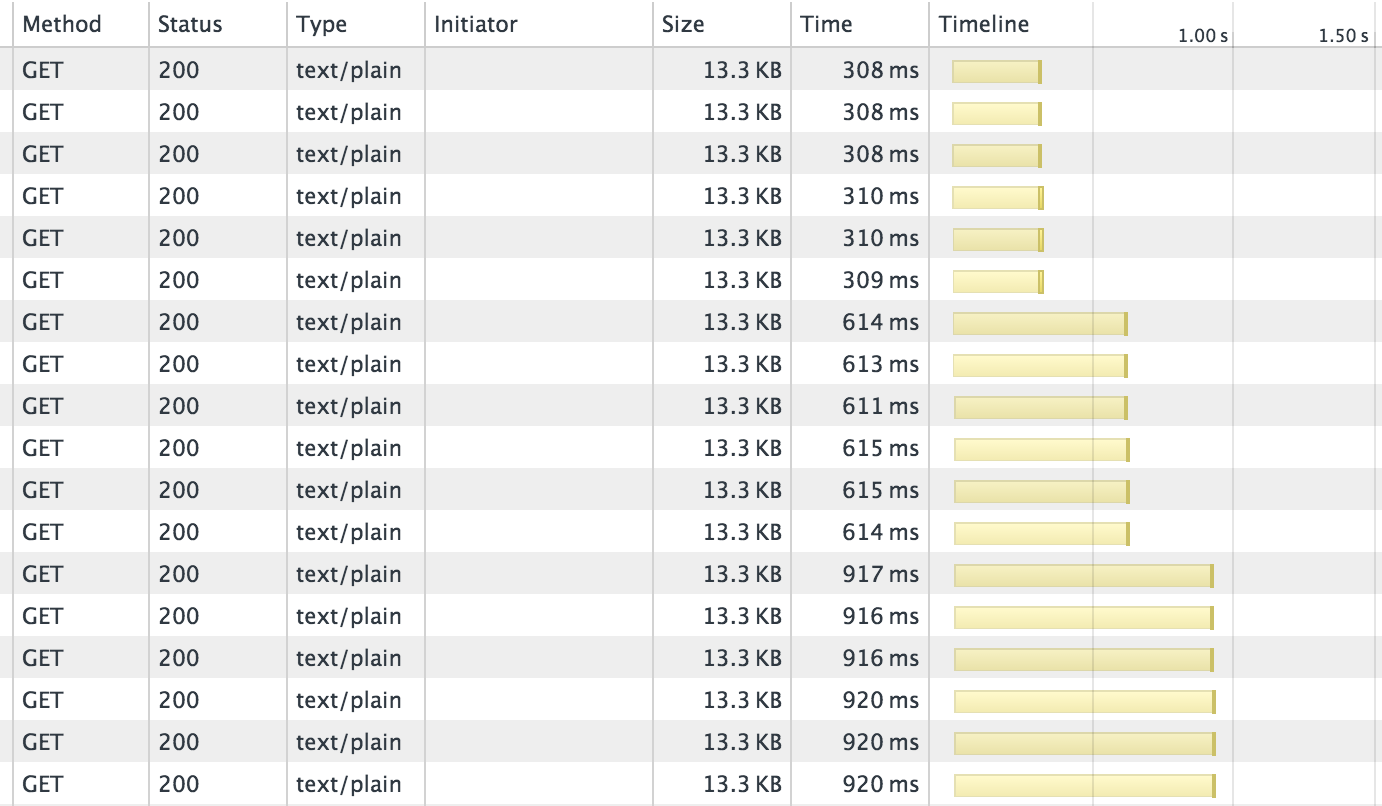
\includegraphics[width=0.9\textwidth]{images/chrome_latency_limit.png}
    \end{center}
  \caption{Chrome developer tools showing how the six TCP connection limit becomes a bottle neck on a connection with 300 ms of latency.}
  \label{fig:tcp_bottleneck}
\end{figure}

We can calculate the total amount of delay caused by latency in our example with the following formula:

\begin{equation}
\mbox{total latency} = \mbox{number of thumbnails} * \frac{\mbox{latency per request}}{\mbox{number of parallel requests}}
\end{equation}

In our example, we fetch 60 thumbnails on a connection which has a latency of 300~ms to the server. Our browser (Google Chrome) can handle six parallel TCP connections which gives us the following equation:

\begin{equation}
\mbox{total latency} = 60 * \frac{300}{6} \mbox{ ms}= 3,000 \mbox{ ms} = 3 \mbox{ seconds}
\end{equation}

If we instead could concatenate these 60 thumbnail requests into one request, and the response would contain all of the thumbnails, then we would only have to pay the latency cost once. This would reduce the total amount of latency by an order of magnitude, from 3,000 ms to 300 ms, since we only have to pay the price for the latency once and not for every six thumbnails.

Other similar approaches to the same problem include CSS Sprites\cite{css_sprites} where a predefined set of images, such as icons, are merged in to one large image file. Individual images are then displayed by rendering parts of the larger image across the website. Note that this approach only works on a predefined set of images since the image merging process is costly and it would therefore not work in the thumbnail example above.

Text-based files such as JavaScript source code files and CSS stylesheets can also be concatenated into larger files during the build process in order to decrease the amount of HTTP requests needed\cite{js_concat}.

As a side-note, it is worth pointing out that increasing the bandwidth of the connection would not resolve this problem as the latency is the only bottleneck in this example. We often focus on increasing the bandwidth as our connections to the internet improve when we perhaps should focus more on the latency instead.

It is not uncommon for browsers to wait idle for 100--150~ms before spending 5~ms actually downloading an image. This means that latency often accounts for 90--95\% of the total waiting time for HTTP requests\cite{latency}. 

\subsection{Chunked responses}
In the previous example where we fetched thumbnails, we often want to display each thumbnail as soon as each individual image has been loaded. This could cause problems now that we are using one concatenated request instead of a separate request for each image. Fortunately we can utilise chunked responses for this.

The HTTP server can utilise chunked transfer encoding in the HTTP responses in order to send the individual thumbnail data in chunks to the client\cite{chunked}. By doing so, images, or any other type of data, can be rendered in the client as soon as each chunk is available, even out of order if necessary. 

This approach, with concatenated requests and chunked responses, has been successfully been implemented at Dropbox in their gallery software implementation\cite{dropbox_chunked}---much in the same fashion as the previous example.

Chunked transfer encoding is the only encoding which HTTP/1.1 clients are required to understand\cite{chunked_required}. This makes it very attractive to use---especially in the use cases where data chunks can be separated in to logical pieces.

\section{Compression}
\label{compression_more}

All requested data, especially text based data, can be compressed before it is sent to the client in order to reduce the transferred data size. A common compression algorithm used together with HTTP requests is GNU Zip (Gzip). Gzip works best on text-based files such as HTML, CSS and JavaScript and has an expected compression rate of 60--80\% when used on text-based files\cite[page 237]{HPBN}.

It is worth mentioning that there are scenarios where Gzip compression applied to very small files can increase the total size because of the Gzip dictionary overhead. This problem can be mitigated by defining a minimum file size threshold\cite{google_gzip}.

As an example, arbitrary user data\footnote{\url{https://gist.github.com/AntonFagerberg/32ddde695fb0e2581176}} for 50 users was created and encoded in JSON format. When this data was requested from a server without compression, the total size of the HTTP request payload amounted to 55,205 bytes of data. By applying Gzip compression to the same data, the content length was reduced to 16,563 bytes of data which amounts to a 70\% space saving. 

\begin{equation}
\mbox{Space Saving} = 1 - \frac{\mbox{Compressed size}}{\mbox{Uncompressed size}} = 1 - \frac{16,563}{55,205} \approx 70\%
\end{equation}

An important thing to note about Gzip compression is that only the payload is compressed in HTTP/1.1\cite{header_compression}. This means that the headers, including cookies, are not compressed which would have otherwise been an additional performance gain. This is one of the improvements which have been addressed in the development of HTTP/2\cite[page 19]{hpbn2}.

\section{Further reading}
\subsubsection{High Performance Browser Networking - What every web developer should know about networking and web performance, Ilya Grigorik, 2013, O'Reilly Media}

The essential book about browser networking performance. It covers many aspects around browser networking and the limitations within the HTTP protocols which are essential to understan in the development of performance increasing API gateways.

\subsubsection{HTTP/2: A New Excerpt from High Performance Browser Networking, Ilya Grigorik, 2015, O'Reilly Media}

A new excerpt from the High Performance Browser Networking book. The new excerpt describes the new features in the HTTP/2 protocol such as the header compression and request/response multiplexing which has to be taken into consideration in API gateways.

\subsubsection{High Performance Web Sites - Essential Knowledge for Front-End Engineers, Ilya Grigorik, 2007, O'Reilly Media}

Techniques for building high performing web sites. These techniques can also be applied inside API gateways.

\subsubsection{Even Faster Web Sites - Performance Best Practices for Web Developers, Ilya Grigorik, 2009, O'Reilly Media}

Follow-up book to High performance Web Sites with additional techniques which can be applied inside API gateways.

\subsubsection{Nine Things to Expect from HTTP/2, Mark Nottingham, 2014, mnot's blog}

A blog post from Mark Nottingham, chair of the IETF HTTP Working Group and a member of W3C TAG, in which he briefly explores nine tings to expect from HTTP/2.

\noindent \url{https://www.mnot.net/blog/2014/01/30/http2_expectations}

\chapter{API gateways in theory}
When developing clients for back-end APIs, you often find that the client's needs and the back-end APIs functionality is not a perfect match. On top of that, different functionality is often required based on whether the client is a mobile application, a desktop application or something entirely different. The way the clients want to use the API can also radically differ based on what kind of product is being developed.

Not being able to optimise the API for each individual client's needs can hurt the clients performance since it has to do a lot of extra work to refit the back-end's model to its own model---but it can also strain the developer who may have to refit the API for each new client.

Changing the back-end API is often not possible, perhaps especially in the enterprise environment where things tend to move slowly. The back-end can be a legacy system where changes are not allowed to take place---it might be impractical to adapt the back-end for different client types without breaking existing clients or the back-end development team might be strained for any other reason.

One approach to mitigate these problems is by utilising an API gateway as a new software layer between the clients and the back-end APIs. By introducing an API gateway, API calls can be modified in many different ways when they are transported between the client and the back-end API.

\section{What is an API gateway?}
An API gateway works on a new layer between the clients and the servers. For an API gateway to be efficient, it has to be able to modify the communication between the clients and the servers, and by doing so, improve the clients and potentially also the servers performance.

The focus in this thesis is to see how the clients can be optimised in terms of performance but also regarding code complexity and developer productivity. Little effort is taken to optimise the server---the goal is however not to put more strain on the server after introducing the API gateway but rather to keep it on the same level as before.

\begin{figure}[H]
  \centering
    \begin{center}
      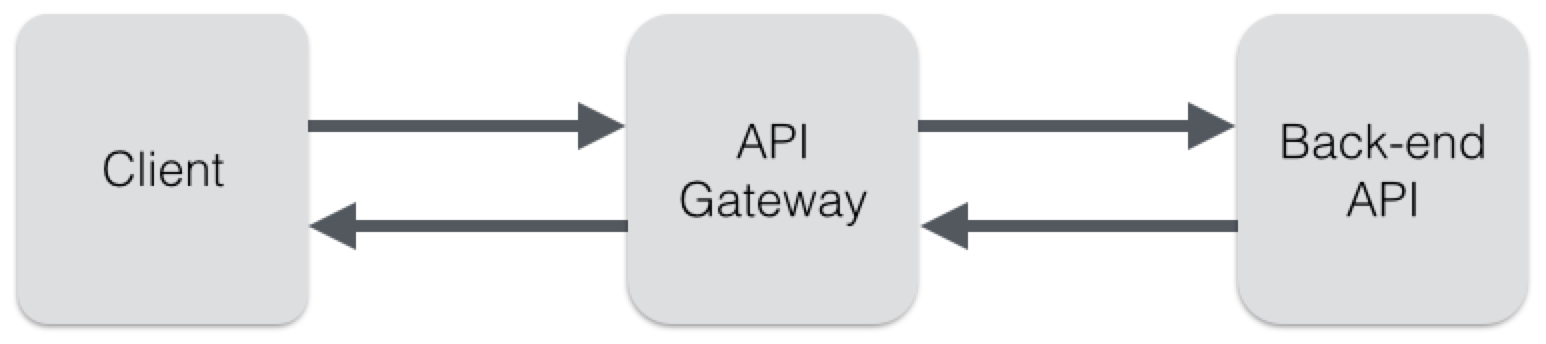
\includegraphics[width=0.9\textwidth]{images/api_gateway.png}
    \end{center}
  \caption{The API gateway is placed as a new separate layer between a client and a back-end API.}
\end{figure}

One might suspect that the amount of code will increase as we introduce yet another software component. However, in many scenarios, the code we write in the API gateway had to be written in the client if the API gateway did not exist. With this reasoning, we can use, to some extent, the same amount of code but gain a lot from just placing it closer to the back-end APIs.

\section{Differing client needs}
We now, perhaps more than ever, have a vast variety of consumer devices such as mobile phones, tablets, desktop computers and other smart devices such as TVs---all of which often utilise the same APIs. One can imagine an API which returns a collection of the latest uploaded images to some service. 

Since the screen size is drastically different on a mobile phone compared to a TV, the number of images the client wants to retrieve from the API can vary a lot. Depending on the type of client which is requesting the data, the API gateway can adapt the number of returned images.

A similar approach has been implemented at Netflix where each client development team write their own \enquote{adaptor} code to fully optimise the underlying API for their client's specific needs\cite{netflix}. This concept works much like how an API gateway works---the main difference being whether the adaptors are actually part of the back-end system or in a new software layer.

\section{Multiple resources and requests}
A client often want to perform many requests simultaneously, either to one or multiple back-end APIs. A typical scenarios is when a user loads a single-page web application for the first time and the application's initial state has to be retrieved. Another typical example is when multiple resources, which are connected in some fashion, has to be loaded.

\begin{figure}[H]
  \centering
    \begin{center}
      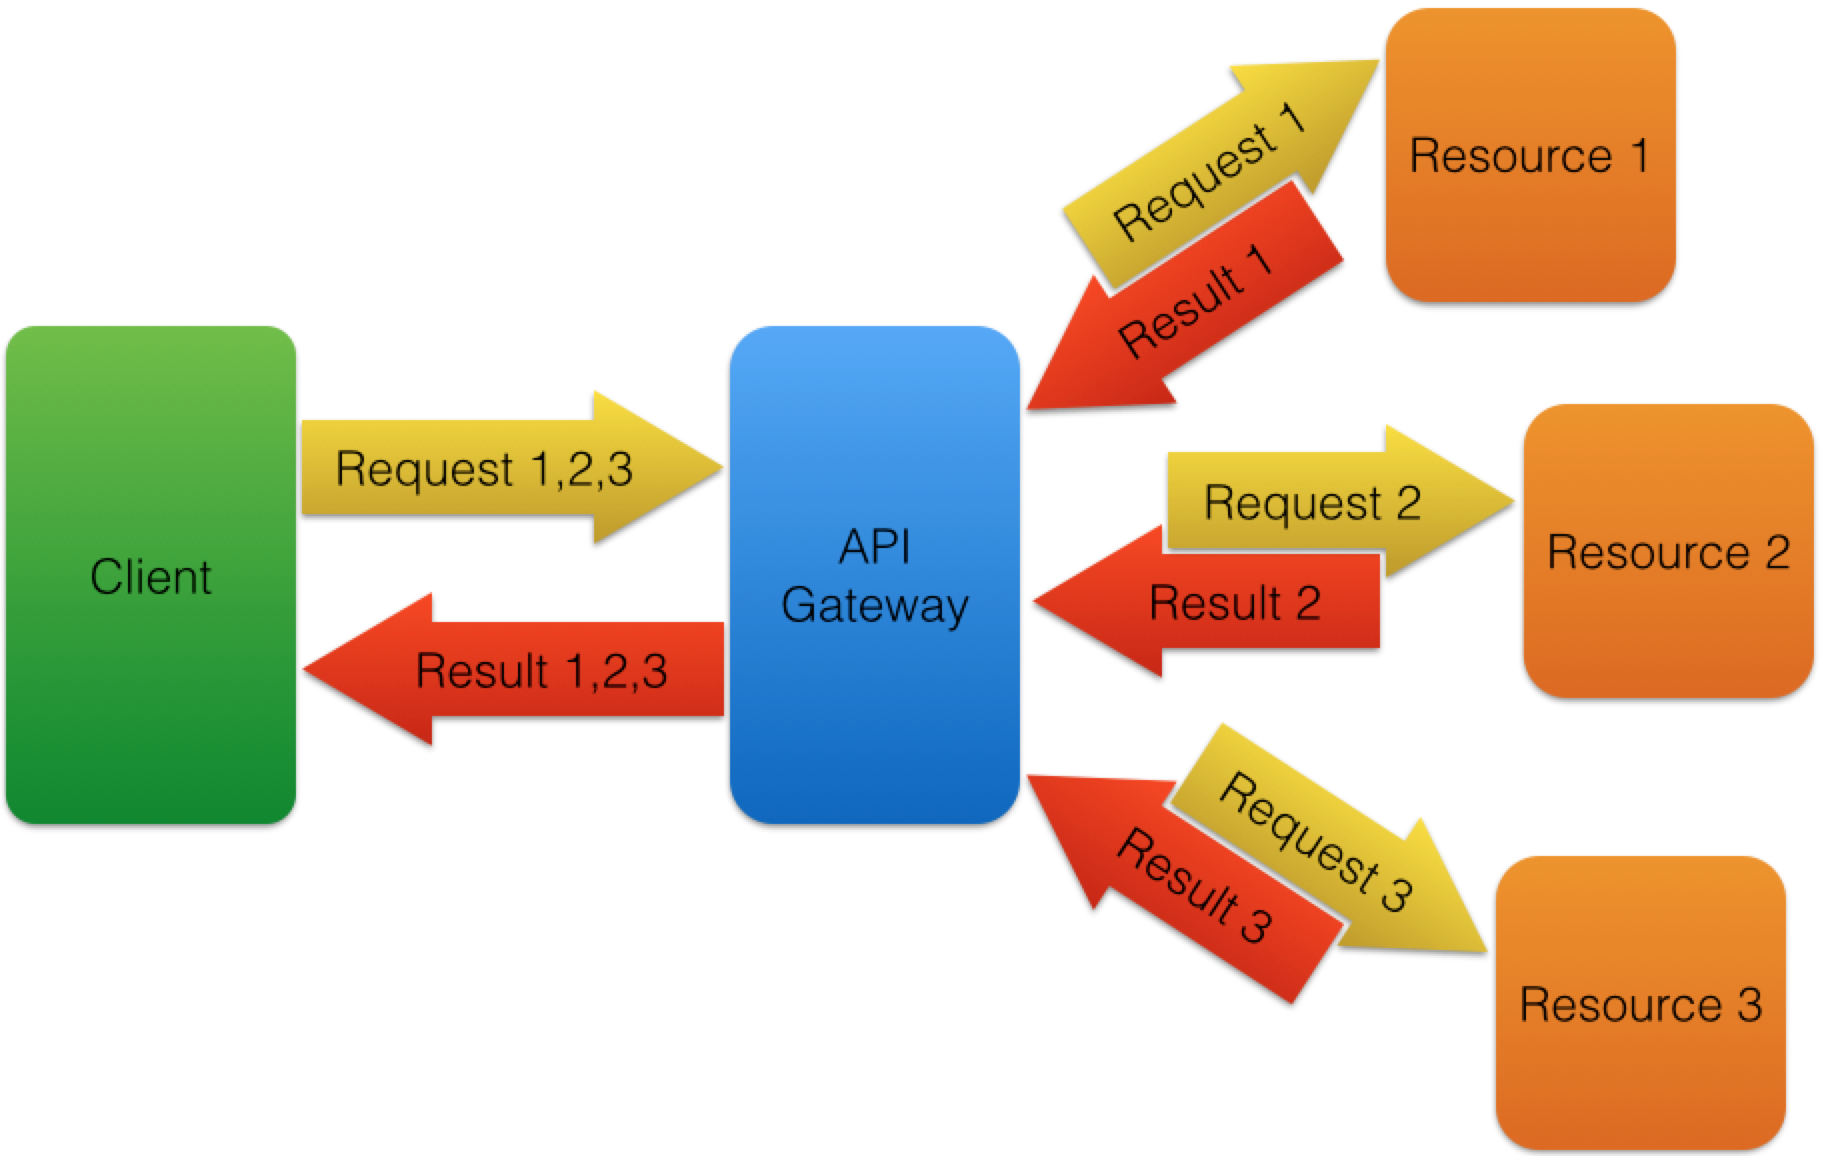
\includegraphics[width=0.9\textwidth]{images/api_gateway_concatenation.png}
    \end{center}
  \caption{The API gateway receives a concatenated request which it distributes to multiple resources, the responses are then concatenated into a single response. The resources can either belong to one or several back-end systems.}
\end{figure}

When working with HTTP requests, there are multiple penalties for executing many requests compared to one concatenated request. These penalties includes the previously mentioned limit of maximum TCP connections (page \pageref{max_tcp}) and the overhead from HTTP headers (page \pageref{headers}). 

We can, by utilising an API gateway to concatenate many HTTP requests, avoid these common problems. Concatenating requests can be seen directly in many modern API designs such as the Facebook Graph API\cite{facebook_batch_requests}---but for the APIs which lacks this feature, an API gateway can effectively mitigate these problems.

\section{Duplicate and unnecessary items}
When requesting data from a back-end API, the responses may contain unnecessary data which the client do not need. In a similar fashion, if a client performs several similar requests, it is possible that all the responses contains some amount of duplicate data. By utilising an API gateway, the results from the back-end API can be modified to remove the items which the different clients do not need.

\begin{figure}[H]
  \centering
    \begin{center}
      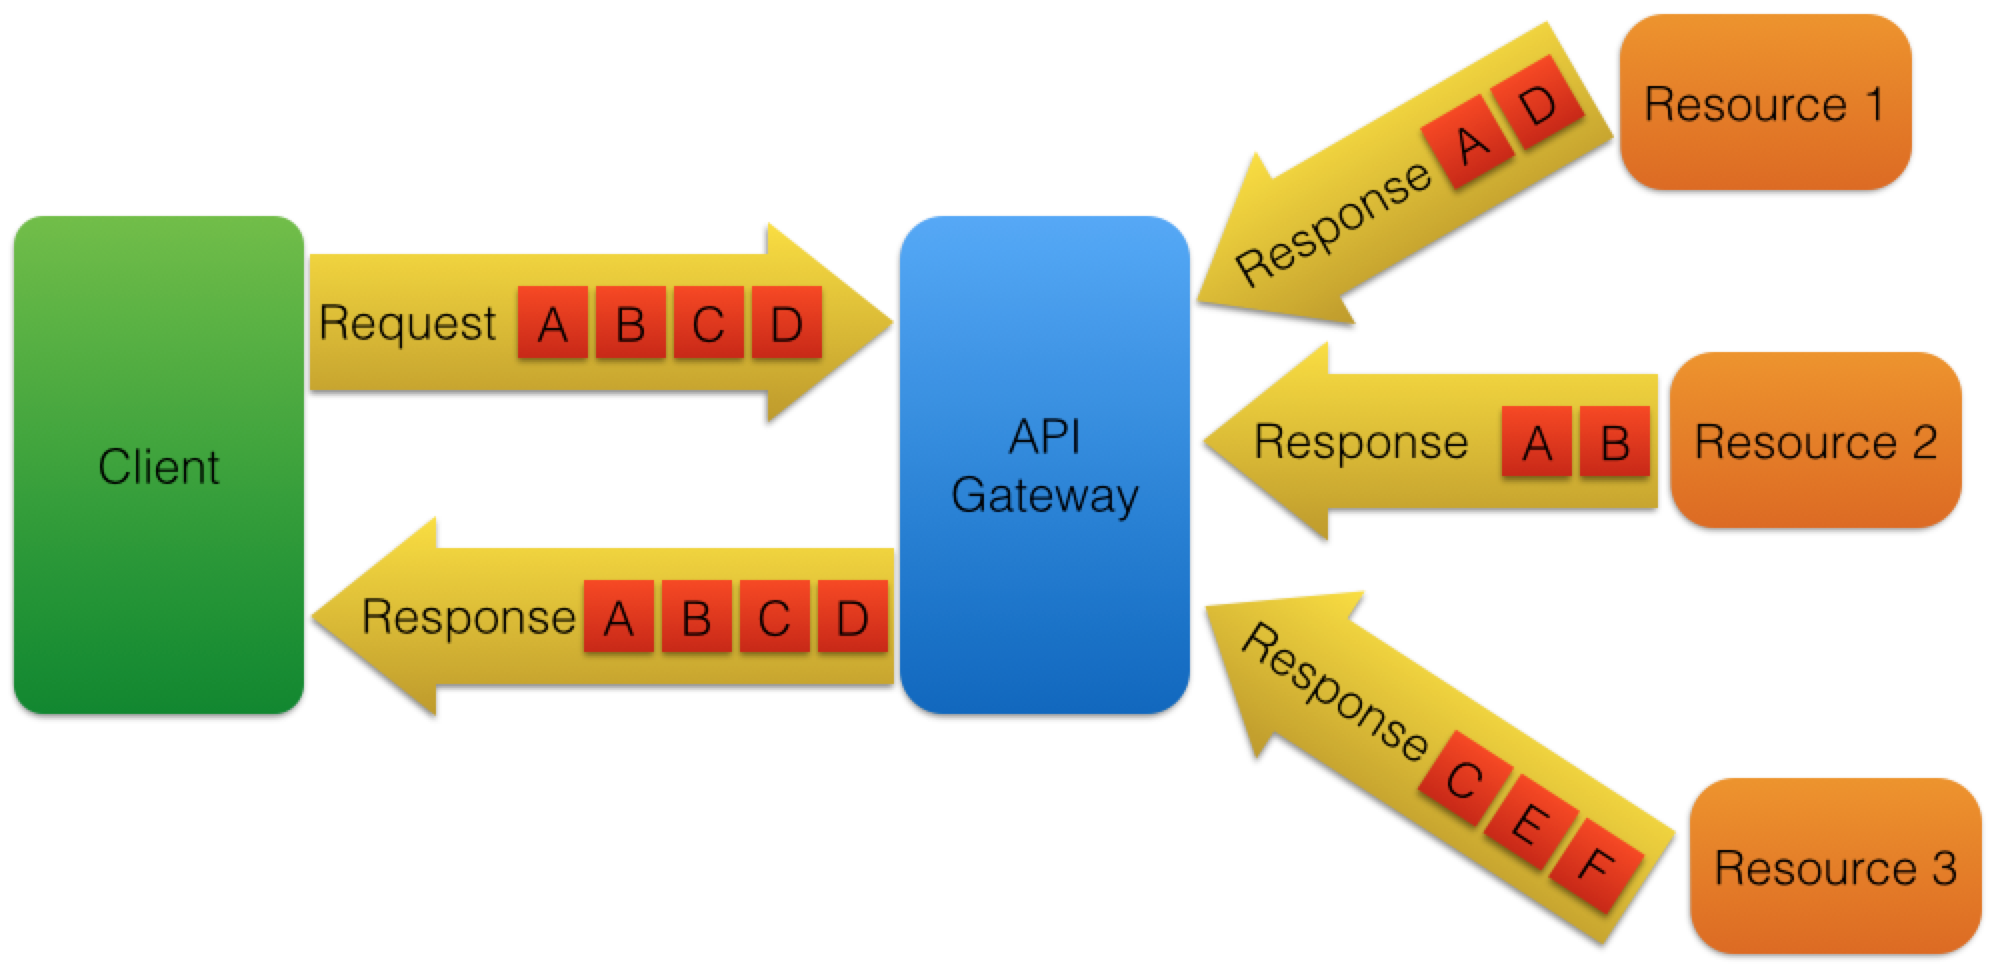
\includegraphics[width=0.9\textwidth]{images/api_gateway_duplicate.png}
    \end{center}
  \caption{The client requests the items A, B, C, D. The API gateway fetches A, D from Resource 1---item A from the Resource 2's response can then be discarded since it is duplicate data. Item E, F from Resource 3 can be discarded since they are not wanted by the client at all. The API gateway can after retrieval respond with just the requested items A, B, C, D.}
\end{figure}

\section{Format transformation}
When working with older legacy systems, the data can be formatted in a way which is not suitable for modern clients. When looking at clients written in JavaScript, many browsers and developers prefer to work with JSON rather than XML since the translation between JavaScript objects to JSON is a 1:1 mapping---more about this on page~\pageref{xml_json}. API gateways can convert the request and response data to a format more appropriate for the requesting client or the responding back-end.

\begin{figure}[H]
  \centering
    \begin{center}
      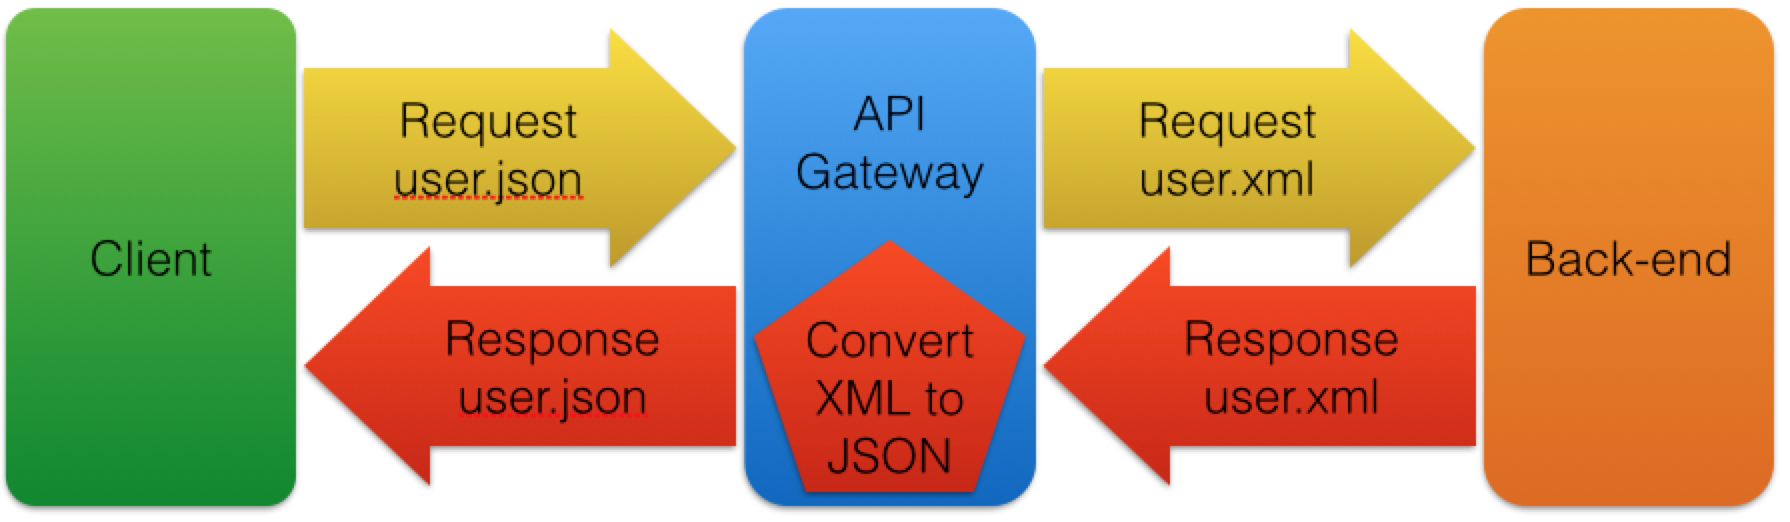
\includegraphics[width=0.9\textwidth]{images/api_gateway_transform.png}
    \end{center}
  \caption{The client requests \enquote{user} in JSON-format. The API gateway fetches \enquote{user} in XML-format from the back-end, converts it to JSON and responds to the client with it.}
\end{figure}

The approach of using an API Gateway has the additional benefit that the conversion code does not have to be rewritten in every client. Rewriting the same conversion code, potentially in a new language or by using a different library, for each client increases the risk of introducing bugs. The reason for this is that different libraries works in different ways even though they solve the same problem---especially when there is no standardised mapping between two formats. Bugs are also introduced as the size of the code base grows such as when the same task has to be rewritten several times\cite[page 521]{code_complete}. 

By performing the transformations in the gateway, the processing work is moved away from the clients which can improve its performance as well as reducing the code size and its complexity.

\section{Pure REST and HATEOAS}
If an API follows the strict rules of REST\footnote{Representational State Transfer, see appendix.}, it must utilise the concept of HATEOAS\footnote{Hypermedia as the Engine of Application State, see appendix.}. Instead of defining and explicitly sharing a collection of end-points which the client can call, it requires the client to discover the resources itself by first performing a GET HTTP request to the APIs root URL. The back-end will respond with all the resources available from the root such as \enquote{users}. The client then has to query the \enquote{user root} to discover which requests can be made in regards to the user resource---and so forth. 

By forcing the client to discover all resources, the client developer has to do a lot of demanding work in the implementation phase\cite[page 62]{AASG}. This approach also introduces a lot of HTTP requests which increases the network traffic significantly.

API gateways can be utilised to transform a \enquote{Pure REST API} with HATEOAS to a simpler API which only follows some of the restrictions put in place by the REST architectural principles. This can significantly lower the amount of traffic between the client and the back-end, which can be a big performance gain, especially in cases such as when there is a high latency between the client and the back-end---assuming that the latency between the API gateway and the back-end is low such as when they are placed inside the same LAN\footnote{Local Area Network, see appendix.}.

\begin{figure}[H]
  \centering
    \begin{center}
      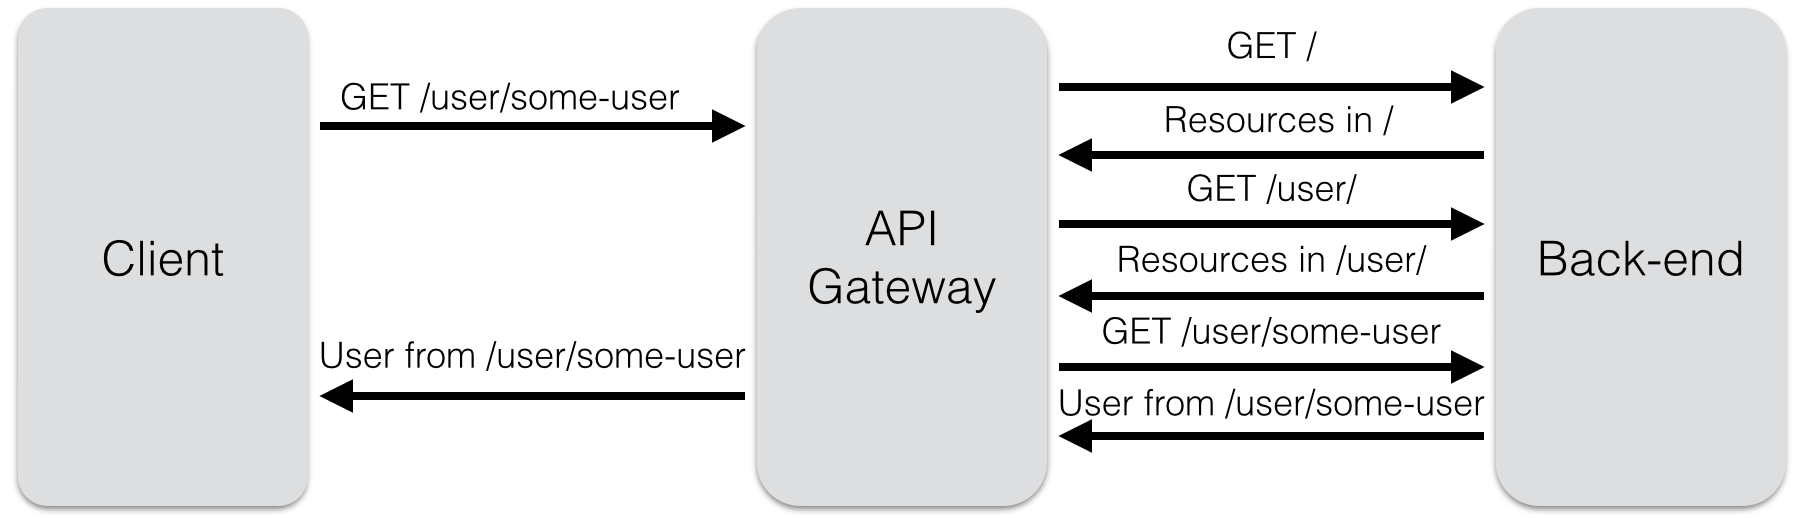
\includegraphics[width=0.9\textwidth]{images/api_gateway_hateoas.png}
    \end{center}
  \caption{The API gateway performs the pure REST HATEOAS communication. At the same, the API gateway exposes a simpler end-point which the clients can call.}
\end{figure}

\section{Compression}
\label{compression}
API gateways can be utilised to compress responses in the cases where no compression is present on the back-end API servers. This can significantly reduce the amount of traffic the client has to receive which increases the performance, especially on mobile devices with low bandwidth. HTTP compression was explored on page \pageref{compression} where it was noted that Gzip has an expected compression level of 60-80\% on text-based media.

\begin{figure}[H]
  \centering
    \begin{center}
      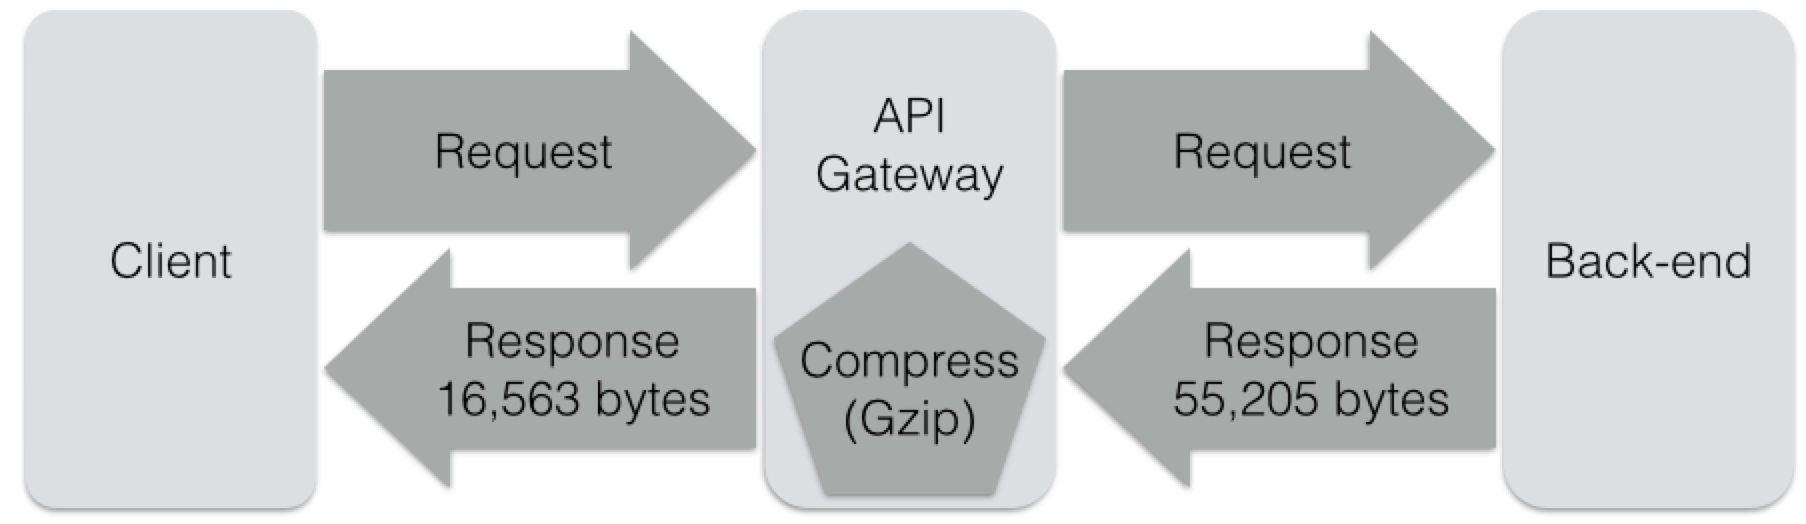
\includegraphics[width=0.9\textwidth]{images/api_gateway_compression.png}
    \end{center}
  \caption{The API gateway compresses the response from the back-end API by utilising the Gzip algorithm. This reduces the response traffic in the client by 70\%. Numbers taken from the example on page~\pageref{compression}.}
\end{figure}

\section{Caching}
\label{caching}
Responses from frequent API calls can be cached using the API gateway in order to reduce the load on the back-end system\cite[page 107]{AASG}. The cache can have a specified lifetime or be invalidated based on certain events. There are several different caching strategies and many popular third-party systems which the API gateway can utilise---caching is a vast and complex topic in itself and is therefore not explored in further detail here.

\begin{figure}[H]
  \centering
    \begin{center}
      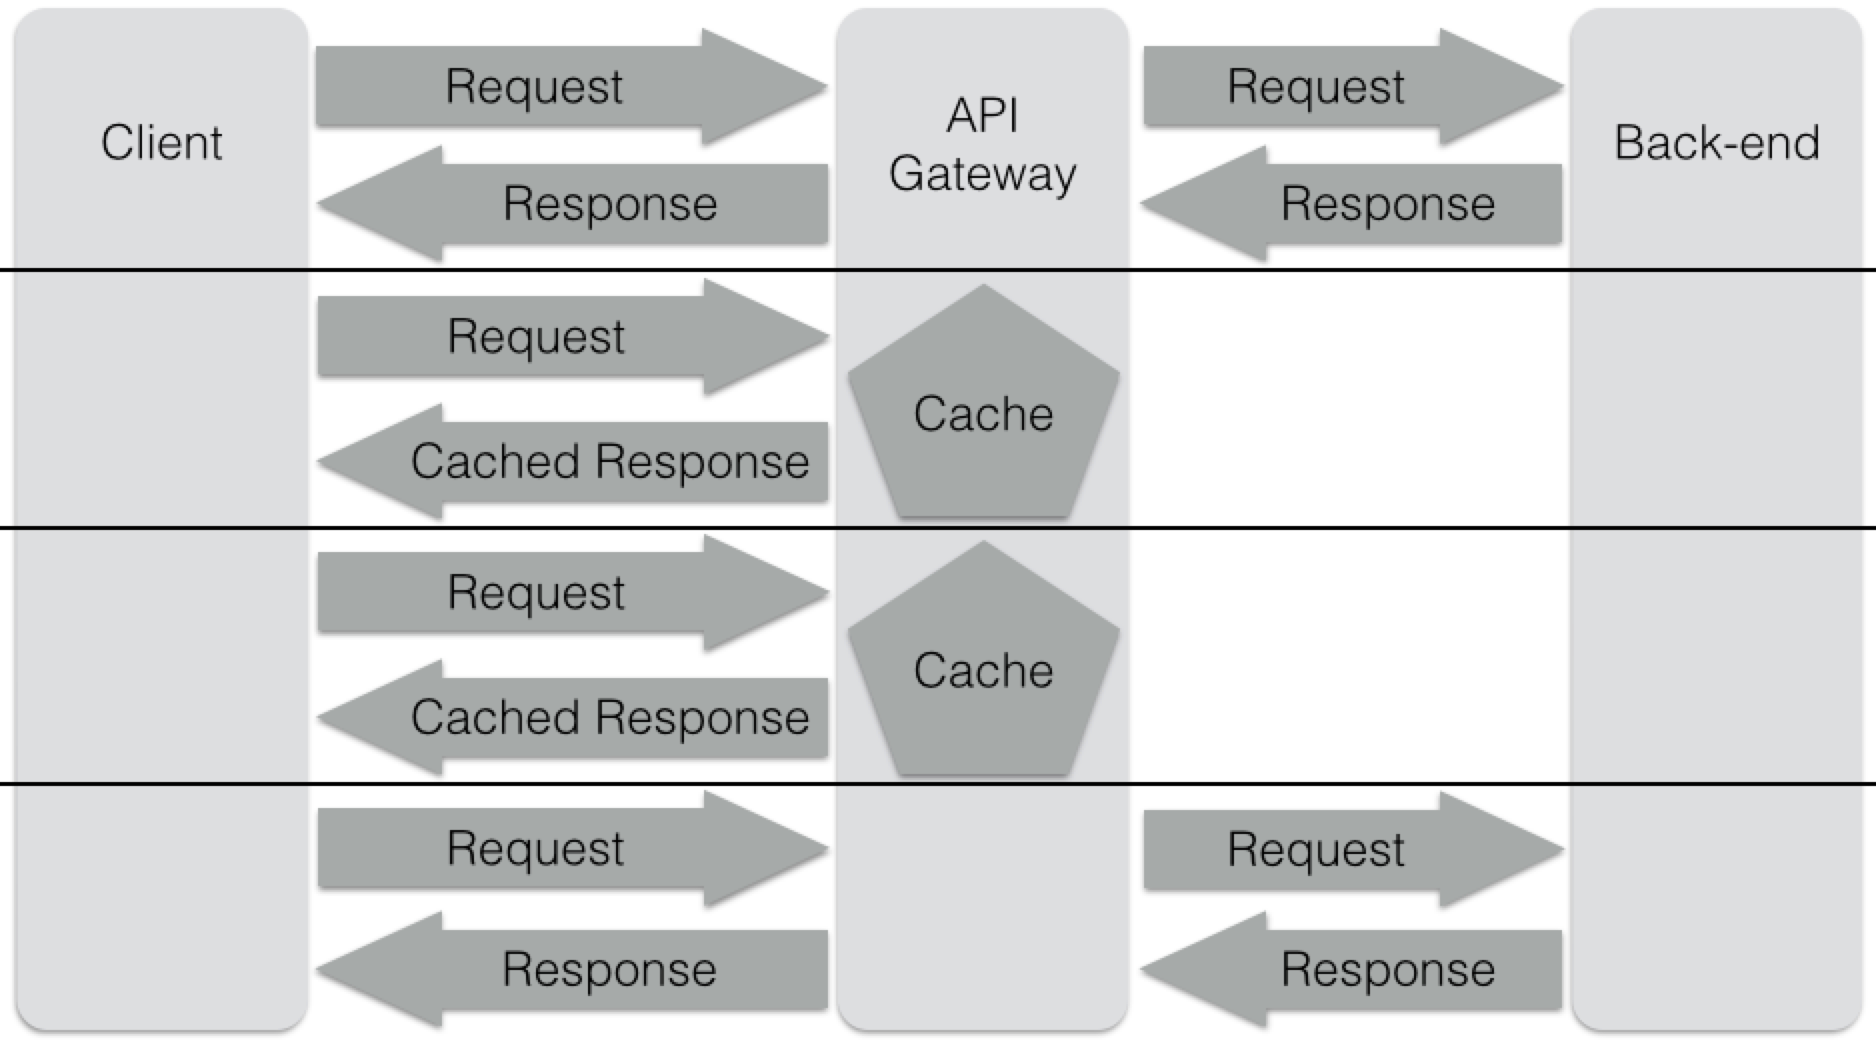
\includegraphics[width=0.9\textwidth]{images/api_gateway_cache.png}
    \end{center}
  \caption{Frequent API calls to the same end-point can be cached in the API gateway to reduce the load on the back-end servers.}
\end{figure}

\section{Decreasing bandwidth and cost}
Cloud providers, such as Amazon\cite{cloud_amazon} and Microsoft\cite{cloud_microsoft}, do not charge for used bandwidth as long as data is transfered between servers in the same cloud regions. When utilising an API gateway in the cloud, bandwidth and its costs, to and from the client, can be reduced by placing the API gateway in the same cloud region as the back-end servers and apply bandwidth saving techniques such as the previously in this chapter mentioned: compression, duplicate \& unnecessary items, pure REST and in some cases even format transformation.

\begin{figure}[H]
  \centering
    \begin{center}
      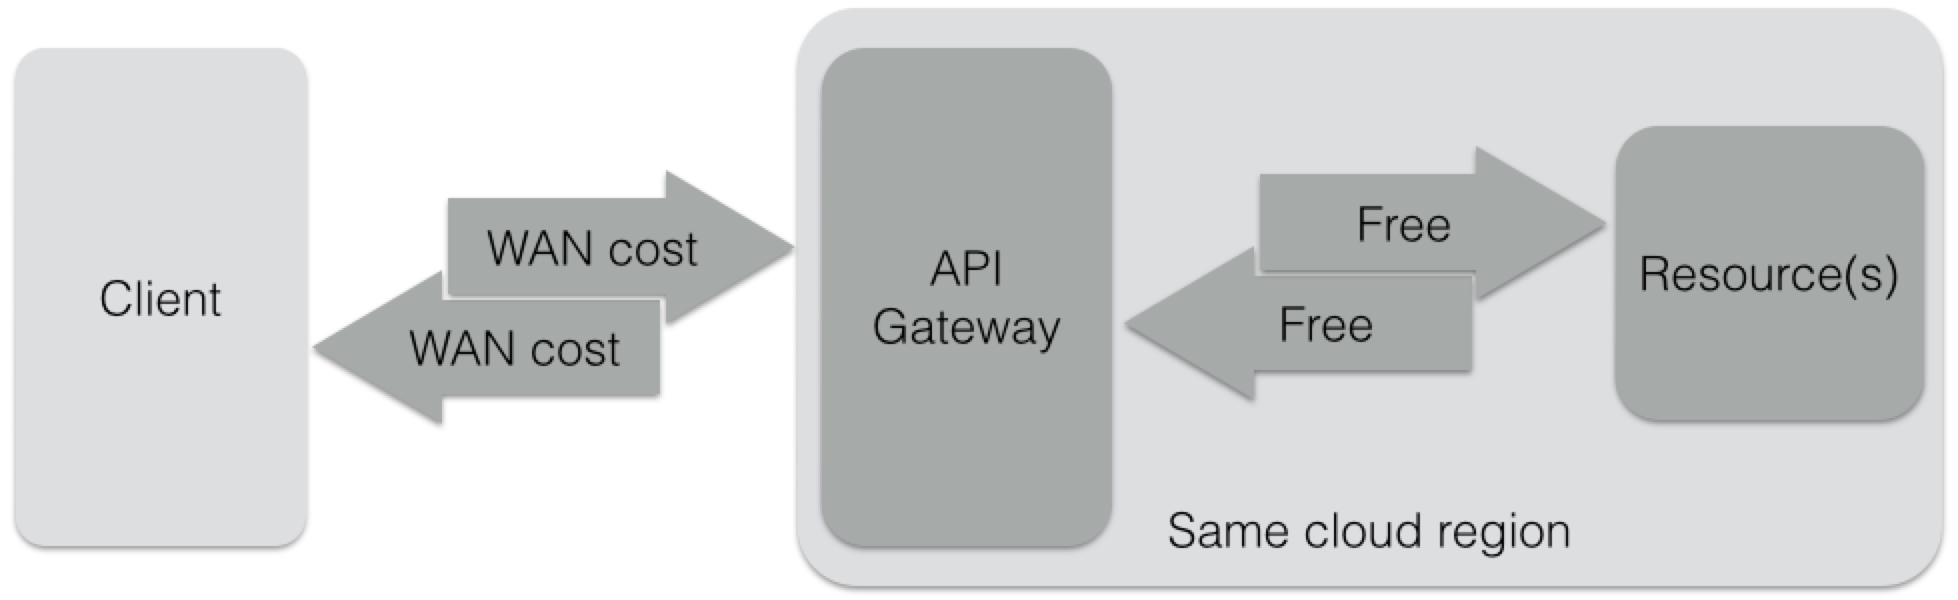
\includegraphics[width=0.9\textwidth]{images/api_gateway_bandwidth.png}
    \end{center}
  \caption{Cloud providers such as Amazon\cite{cloud_amazon} and Microsoft\cite{cloud_microsoft} charges based on whether the traffic is over WAN or in the same cloud region.}
\end{figure}

\section{Secure point of entry for private networks}
Corporations usually uses several internal services with APIs that are protected inside a private network. A VPN\footnote{Virtual Private Network, see appendix.} can be utilised to give clients on the outside access to services inside the private network. A VPN can however have the undesired side effect of exposing to much of the private network to the external client machines.

Another approach to solve this is to place an API gateway inside the DMZ\footnote{DeMilitarized Zone, see appendix.} of the private network. By doing so, external clients can access the API gateway as a single point of entry for all internal APIs. The API gateway can be configured to only expose a predefined collection of the internal APIs and proxy them to the appropriate external clients.

\begin{figure}[H]
  \centering
    \begin{center}
      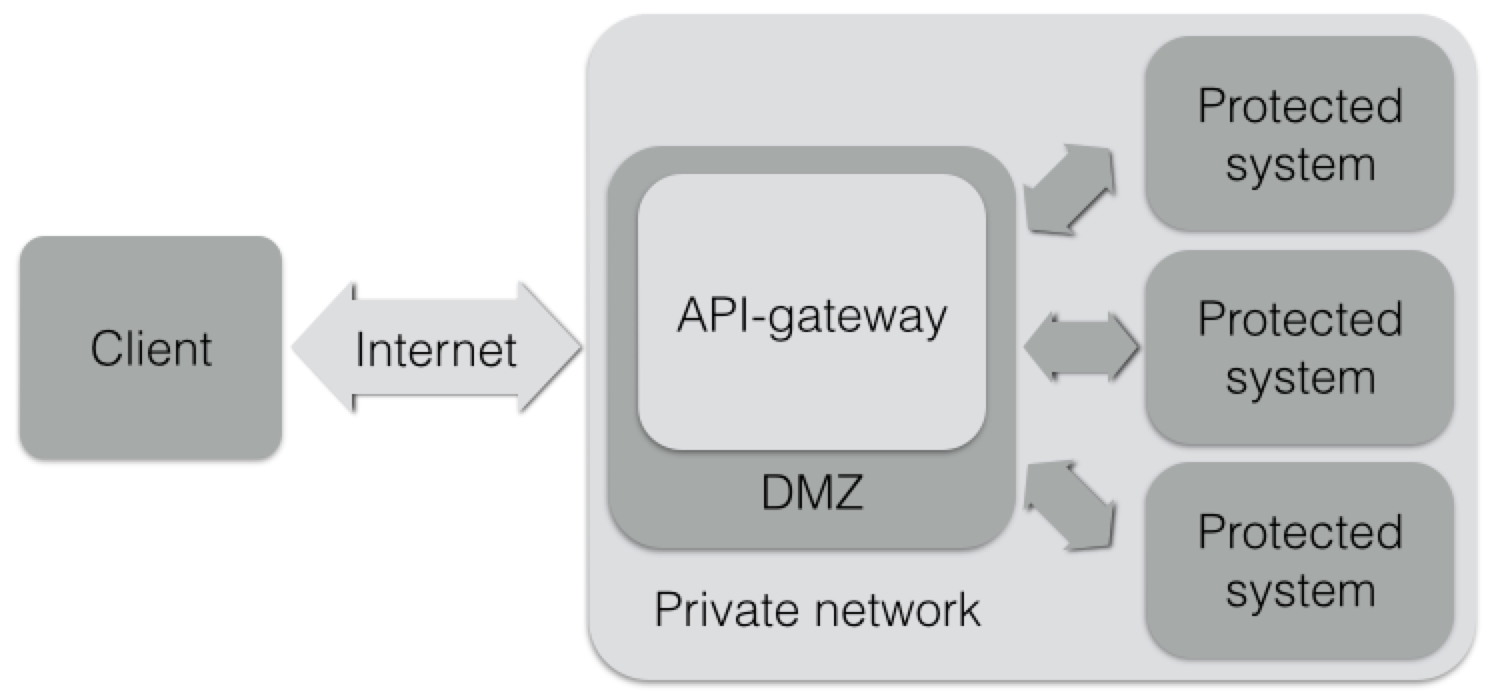
\includegraphics[width=0.9\textwidth]{images/api_gateway_dmz.png}
    \end{center}
  \caption{An API gateway used as a secure way of exposing internal services in a private network to the outside world.}
\end{figure}

\section{Latency}
One important goal of an API gateway is to reduce, or at least not significantly increase, the latency experienced in the communication between the client and the back-end server. Because of this, the placement of the API gateway from a network point of view is very important. (In all of the following scenarios, we treat LAN latency as negligible which should be a fair assumption.)

The first approach we look at is placing the gateway on the same LAN as the client. Placing the API gateway on the same machine as the client is rarely possible or practical---it complicates updating the gateway and defeats much its purpose of introducing a new layer between the client and server. 

Placing the API gateway inside the same LAN as the client can be a good solution, for example when it is used inside a corporation's private network. The constraint with this approach is that no outside clients, such as smartphones not connected to the internal network, will be able to avoid the extra latency introduced over WAN\footnote{Wide Area Network, see appendix.}---or may not be able to connect to it at all based on the LAN security. This is however an approach which does not introduce double latency, but it does not decrease it either.

The second approach is to place the API gateway as a separate application in its own cloud or on a LAN separated from the back-end and client. While this may be the only solution for certain hosting setups, this introduces the problem of double latency. Since the TCP-packets has to go through two WAN connections, both of them can introduce a substantial amount of latency which can worsen the response times.

Finally, the third approach is to place the API gateway on the same LAN as the back-end system. This is in many cases the best approach as it avoids the problem regarding double latency while it at the same time provides access for external clients and introduces flexibility in regards to updates. 

The problem with double latency can however arise, and be unavoidable, if the API gateway is communicating with several back-end systems which are placed on different LANs. In such a scenario, several factors have to be considered before deciding which LAN to place the gateway in. Such factors include which back-end API has the most traffic, bandwidth costs between LANs, the latency between the different LANs and so forth.

\begin{figure}[H]
  \centering
    \begin{center}
      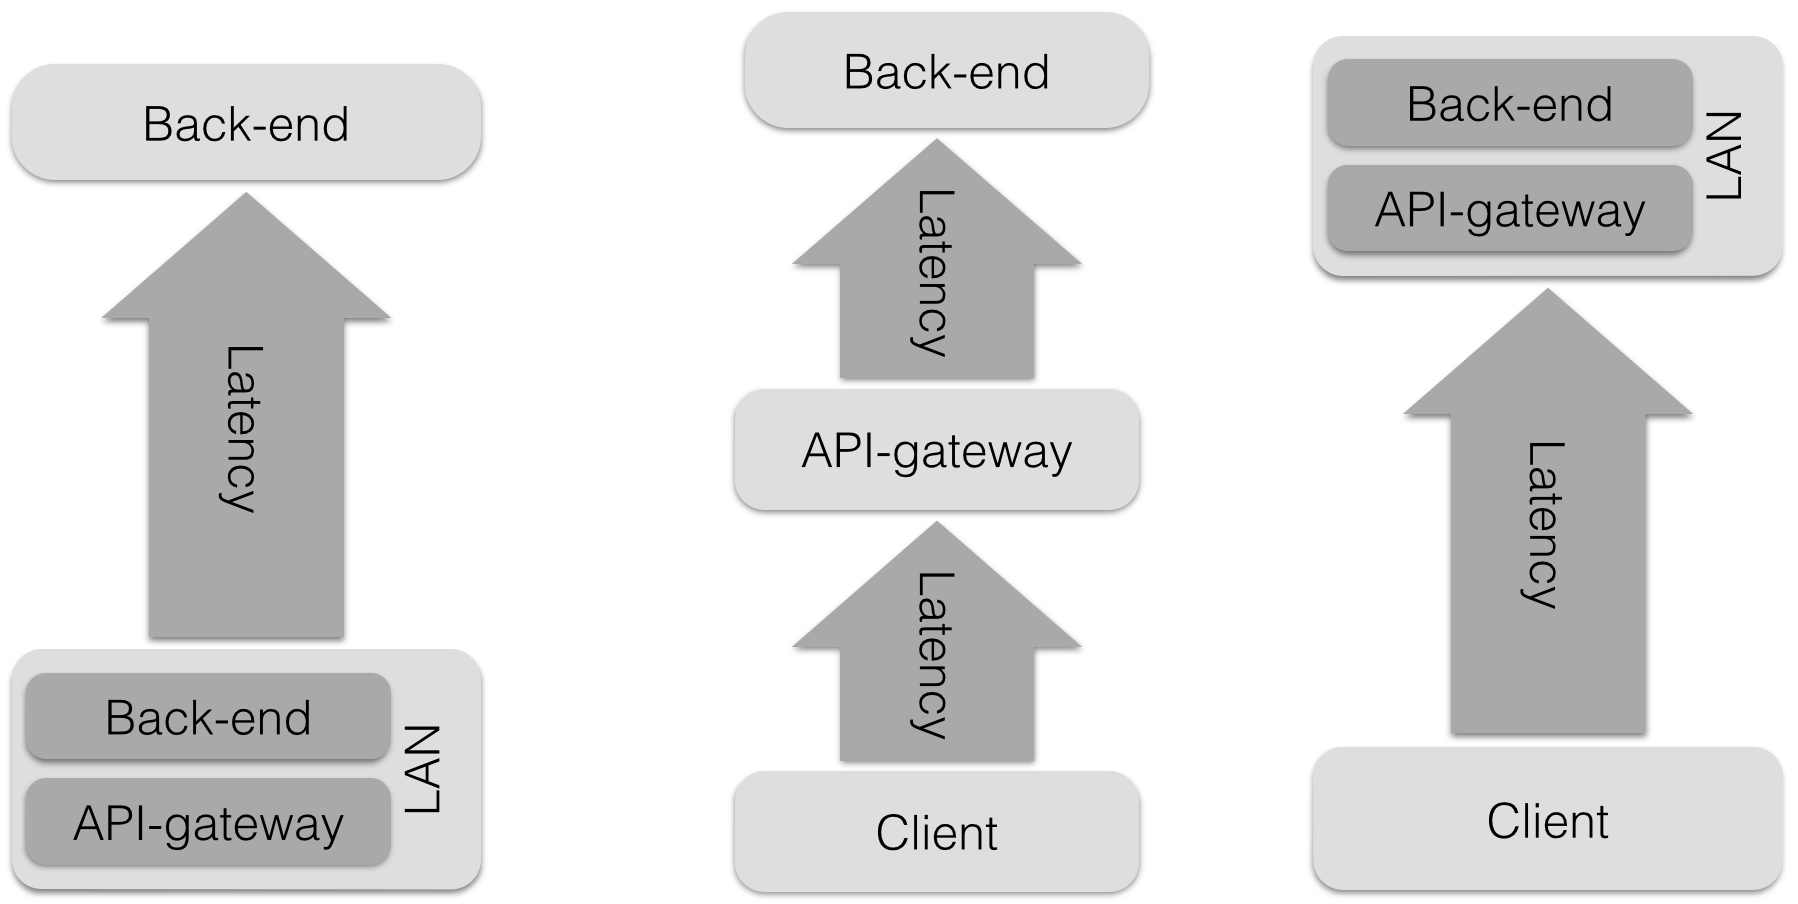
\includegraphics[width=0.9\textwidth]{images/api_gateway_latency.png}
    \end{center}
  \caption{How latency affects the different placement strategies for the API gateway.}
\end{figure}

\section{Error handling}
An API gateway should be able to handle potential errors with different strategies. In the simple scenarios where a single request is proxied and potentially transformed, the API gateway can chose to either resubmit the failing request to the back-end API a number of times, potentially after a small delay, or to simply relay the error to the client.

Deciding what to do in more complex cases where several requests are concatenated or transformed together is much harder. The developer of the API gateway's end-point has to decide if a partial result is relevant for the client or if one failure should invalidate the entire combined result.

Deciding to invalidate the entire result based on one request failure is problematic if the API gateway uses chunked responses. Ideally, the API gateway want to transmit data to the client as soon as it is available but since chunks can not be retracted, the API gateway either has to wait for all back-end results to arrive before responding or introduce some kind of an error chunk which tells the client to discard the previously sent data.

The API gateway developer has to decide whether to handle much of the error complexity in the API gateway itself or delegate this responsibility to the client. These factors has to be considered on a case to case basis---there is no correct answer.

\section{Security---authentication \& authorisation}
\label{sec:security}
API gateway security is, like all security scenarios, a very complex problem. All but the very simplest of cases should be solved outside the implementation of the gateway itself. What makes an API gateway complex from a security point of view is the fact that an end-point exposed from the API gateway can communicate with several back-end systems, all of which can utilise different authentication and authorisation protocols. Because of this, a single sign-on service provided outside the API gateway itself is a good approach for the more complex setups which communicates with several back-end systems.

Any further in-depth discussion regarding this topic is outside the scope of this thesis and has therefore been excluded intentionally.

\section{Conditional back-ends}
By utilising an API gateway, several different back-ends can be exposed as one single end-point. If we, for example, wanted to provide an API with weather reports from Sweden and Denmark but we have noticed that two different back-end APIs provide better reports for each country---one is better for Denmark and one is better for Sweden. With an API gateway, we can translate the incoming API-calls to the format required by the different back-ends and delegate the call based on certain inputs such as from where the API-call is made.

\section{Rate limiting}
API gateways can mitigate traffic spikes on back-end services by implementing a rate limit for API-calls. This can usually be done in many different ways as seen in Azure\cite{azure_rate_limit} and Apigee\cite{apigee_rate_limit}. Rate limiting strategies include a global rate limit, a per client rate limit or a per token rate limit. This functionality is often used from a business perspective where a certain number of calls are free but a fee has to be paid for subsequent calls.

\section{Support from old API versions}
It happens that API developers make changes which break backward compatibility when moving on to newer improved versions of the API. Fields can be added, renamed or removed. In such scenarios, old clients may be forced to update in order to work with these breaking API changes.

Instead of rewriting many of the already released clients to fit the new API-version, an API gateway can, in some cases, be used to translate the new API format back to the old one. How feasible this is depends on what kind of changes that have been introduced and whether they are destructive or not.

\section{Analytics}
API gateways are in a perfect position to collect data that can be used for analytics. This is because the API gateway is able to monitor all the traffic between the clients and the back-ends. 

\vspace{5mm}

\noindent API gateways can collect a lot of analytic data from HTTP requests and responses such as:
\begin{itemize}
	\item Client technology: the browsers user-agent which is sent with request headers is one way to collect a variety of data. The user-agent normally includes the browsers name and version, rendering engine, computer architecture and operating system.
	\item Request-response time for both the client and each individual back-end API calls.
	\item Latency from different back-end APIs.
	\item Geolocation from the HTML 5 geolocation API\cite{html5_geolocation} or by geolocating the requesting IP address.
	\item Errors and failure rates for the back-end servers.
	\item Invalid client requests.
	\item Traffic peak hours.
	\item Suspicious client behaviour such password or denial of service attacks.
\end{itemize}

\noindent Since performance is usually a top priority in API gateways, the collected data should preferably be delegated, stored and processed using a third-party analytics engine.

\section{Load balancing}
API gateways can be used as load balancers to distribute workloads across multiple back-end systems. This can be achieved by implementing different scheduling algorithms---either by doing a simple round-robin or by implementing a more complex algorithm which takes additional factors into account such as the back-end systems reported load, response time, geolocation and so forth.

\section{Related works}

\subsubsection{Netflix API}
Netflix has applied a concept, similar to API gateways, where each client's team develop their own end-points adapted to the client's specific needs.

\vspace{5mm}

\noindent Optimizing the Netflix API, Ben Christensen, 2013, The Netflix Tech Blog

\noindent \url{http://techblog.netflix.com/2013/01/optimizing-netflix-api.html}

\vspace{5mm}

\noindent The Netflix API Optimization Story, Jeevak Kasarkod, 2013, InfoQ

\noindent \url{http://www.infoq.com/news/2013/02/netflix-api-optimization}


\subsubsection{Managing API Performance, Apigee}
Apigee, who works with API tool development, have put together a collection of articles with focus on optimising API performance in common scenarios which are also applicable in API gateways.

\vspace{5mm}

\noindent Managing API Performance, Apigee

\noindent \url{http://apigee.com/docs/content/managing-api-performance}

\chapter{Rackla: API gateway framework}

The framework Rackla\footnote{\url{https://github.com/AntonFagerberg/rackla}} was developed in order to better understand, and be able to rapidly develop, custom API gateways. Existing API gateway technologies, such as Microsoft Azure API Management\cite{azure_api_management}, Apigee Edge\cite{apigee_edge} and IBM API Management\cite{ibm_api_management}, mainly focuses on expanding existing public APIs from a business point of view with focus on monetisation, security and BaaS (backend as a service) using drag-and-drop graphical interfaces. 

Rackla's focus, on the other hand, is from a pure technical point of view. Its goal is to help developers create their own custom API gateways programatically with a high degree of freedom and a small amount of abstractions which otherwise could limit the use cases.

\section{Technologies: language and libraries}
\subsection{Elixir}
Elixir is a functional language designed for building scalable and maintainable applications which run on the Erlang Virtual Machine. The Erlang VM is known for running low-latency, distributed and fault-tolerant systems while also being successfully used in web development\cite{elixir}. We consider all of these properties important when developing a successful API gateway.

Other important factors for choosing to use the language Elixir in this framework is the pipe operator, the asynchronous behaviour defined by Elixir processes and the functional programming aspect of the language.

\subsection{The pipe operator}
An important concept used in Elixir is the pipe operator: \lstinline{|>}. The pipe operator takes the result from the expression on the left side of the operator and \enquote{pipes} it into the first argument of the right hand side function. People who are accustomed to Unix may see a similarity to the Unix pipe operator: \lstinline{|}.

\vspace{5mm}

\noindent As an example, we can take a look at the following nested and hard to read code. The code will take a list of all integers from 1 to 100,000, multiply all the integers with 3, remove all even numbers and finally summarise them:

\begin{figure}[H]
  \centering
\begin{lstlisting}[breaklines=true,frame=single]
Enum.sum(Stream.filter(Stream.map(1..100_000, &(&1 * 3)), odd?))
\end{lstlisting}
  \caption{Elixir code written without the pipe operator.}
  \label{fig:no_pipe}
\end{figure}

\noindent The code from the figure above can be rewritten using the pipe operator which results in a more easily read version:

\begin{figure}[H]
  \centering
\begin{lstlisting}[breaklines=true,frame=single]
1..100_000 |> Stream.map(&(&1 * 3)) |> Stream.filter(odd?) |> Enum.sum
\end{lstlisting}
  \caption{The same code as seen in Figure~\ref{fig:no_pipe} expressed with the pipe operator.}
\end{figure}

Another benefit of using the pipe-operator is that it makes you reason about the code in a more structured way. When you read it, you might say: \enquote{First I have the range of numbers, then I map over it, then I filter them, then I sum them}---which corresponds to how the code is written.

The pipe operator is an important part in how Rackla works as it pipes requests to a response, potentially through transformations along the way. For developers who are not accustomed to Elixir, the minimalistic syntax used inside Rackla can make it look like an easy to read DSL (Domain Specific Language) in which they can expose end-points and pipe requests to the clients without writing a lot of boilerplate code.

\subsection{Elixir processes}
Processes are Elixir's term for utilising the \enquote{actor model} as its concurrency model. In Elixir, processes are extremely lightweight (in comparison with operating system processes) which means that it is not uncommon to have thousands of them running simultaneously. Elixir processes run concurrently, isolated from each other and can only communicate with message passing\cite{elixir_processes}.

\subsection{Plug}
Plug is a specification for composable modules in between web applications---but also as connection adapters for different web servers in the Erlang VM\cite{plug}. In Rackla, Plug is utilised for exposing end-points to which the client can send requests, and a as a way for the API gateway to send responses back to the clients over the HTTP protocol. An additional benefit of using Plug is that already existing third-party code for handling things like cookie management and cross-origin requests can be reused inside Rackla.

\subsection{Hackney}
Internally, Rackla uses the Erlang HTTP client library Hackney\cite{hackney} to send HTTP requests to back-end systems. Hackney is only used internally and it is therefore abstracted away from the Rackla framework users in order to simplify the API gateway development and ensure that Hackney can be removed or replaced in future versions if necessary.

\section{Rackla overview}

\subsection{Pipeline}
A pipeline is the result from using the pipe operator to tie the different functions together. The goal, when writing an API gateway using Rackla, is to describe each end-point as a sequence of steps defined as a pipeline. The simplest scenario is to proxy a request within the API gateway---that is to relay a request without modifying it. We can do that by first defining a URL to call, pipe it to the request function and then pipe it to the response function:

\begin{figure}[H]
  \centering
\begin{lstlisting}[breaklines=true,frame=single]
"www.example.com"
|> request
|> response
\end{lstlisting}
  \caption{A simple proxy which relays the entire payload untouched.}
\end{figure}

\subsection{Monads and Functional programming}
A new type, which can be passed between the different functions, has to be defined in order for the pipeline to work---but also for letting us reason about it. This type has to be able to handle any number of requests asynchronously while still enable us to transform the eventual results before they are sent to the client.

With these constraints, a new type was defined with inspiration taken from the concept of monads (a monad is a structure, often used in functional programming, which represents computations as a sequence of steps).

The new \lstinline{Rackla} type defines what it means to chain operations together using well established concepts commonly found in functional programming such as \lstinline{map}, \lstinline{flat_map} and \lstinline{reduce} with focus on still being asynchronous.

To illustrate this, we can use Rackla to request two images over HTTP, transform the image's binary data by applying a Base64 encoding to them and finally responding to the client with the encoded data:

\begin{figure}[H]
  \centering
\begin{lstlisting}[breaklines=true,frame=single]
["url-to-image-1", "url-to-image-2"]
|> request
|> map(&Base.encode64/1)
|> response
\end{lstlisting}
  \caption{Asynchronously transforming two images requested over HTTP to Base64 encoded data.}
    \label{fig:map}
\end{figure}

It is important to point out that it is the new \lstinline{Rackla} type that allows this pipeline to be fully asynchronous---the order of the response chunks sent to the client will depend on which of the URLs that is responding first and which of the Base64 encodings is performed the fastest. It can very well be the case that one Base64 encoded image has been fully sent to the client while the other image is still being requested in the API gateway.

\subsection{Function overview}
In this section we will go through and explain the most common functions defined in the Rackla framework. These functions enable us to build very flexible and powerful API gateways.

\subsubsection{Request}
The function \lstinline{request}, in the simple case, takes one or many URLs as strings and returns a \lstinline{Rackla} type. The data eventually contained inside the \lstinline{Rackla} type will correspond to either the results from the HTTP requests or error tuples if any error occur such as DNS lookup failures, non-responding back-end or thrown exceptions.

More advanced HTTP requests can be executed by instead passing one or many \lstinline{Request} types to the \lstinline{request} function. By using a \lstinline{Request} type, we can define which HTTP verb to use such as GET or POST, what timeout limits we want to use and how we want to handle insecure SSL connections. We can also define custom request headers and attach a request body (payload) to each individual request.

In addition to this, we can in the \lstinline{request} function define if we want the \lstinline{Rackla} type to contain just the response body, the HTTP responses payload, or a \lstinline{Response} type containing, in addition to the response body, the response status code and response headers.

\subsubsection{Just}
The function \lstinline{just} takes any existing type and encapsulates it inside a Rackla type. This function is useful when mixing already available data with eventually available data from HTTP requests.

\subsubsection{Response}
The function \lstinline{response} takes a \lstinline{Rackla} type and converts the underlying types to an HTTP response and sends it to the client. In order to conform to the asynchronous nature of Rackla, we only use chunked responses\cite{chunked}. We can pass in options in order to customise the response, available options are: \lstinline{json} which automatically encodes the response as a JSON data structure, \lstinline{compress} which compresses the response using GZip compression, \lstinline{sync} which guarantees that the responses are sent in a deterministic order, \lstinline{status} which defines the response's status code and \lstinline{headers} which defines the headers that will be sent with the HTTP response.

\subsubsection{Map}
The function \lstinline{map} is used in order to transform the contents inside the \lstinline{Rackla} type from one type to another type. As an example, we saw in Figure \ref{fig:map} that we can apply a Base64 encoding to each individual image's data from many HTTP requests, contained inside a single \lstinline{Rackla} type.

\subsubsection{Flat map}
The function \lstinline{flat_map} works like \lstinline{map} with the exception that the returned type inside its anonymous lambda function has to be a new \lstinline{Rackla} type. The naive approach is to wrap the returned type using \lstinline{just}, but a more appropriate usage is to utilise this function when you want to initiate another \lstinline{request} pipeline inside a transformation.

\begin{figure}[H]
  \centering
\begin{lstlisting}[breaklines=true,frame=single]
"example-url"
|> request
|> flat_map(fn(response) -> 
	"url-get-more-info-#{response}" 
	|> request 
end)
|> response
\end{lstlisting}
  \caption{A new \lstinline{request} pipeline can be constructed inside the \lstinline{flat_map} function.}
\end{figure}

In the figure above we make an HTTP request to an end-point which will return some response. By using \lstinline{flat_map}, we can create one or more additional requests from the received response by creating a new \lstinline{request} pipeline inside the \lstinline{flat_map}'s anonymous lambda function. This enables us to define recursive request structures which later boils down to a single response.

\subsubsection{Reduce}
The function \lstinline{reduce}, or sometimes called \lstinline{fold}, is a way to take a collection of values and \enquote{reduce} them into to a single value. Rackla provides a \lstinline{reduce} function which reduces the values contained inside its own \lstinline{Rackla} type into a single value (still contained inside a \lstinline{Rackla} type).

\begin{figure}[H]
  \centering
\begin{lstlisting}[breaklines=true,frame=single]
Enum.reduce([1,2,3], &(&1 + &2))
\end{lstlisting}
  \caption{Illustration of how the \lstinline{reduce} function works inside the built in \lstinline{Enum} module in Elixir---the reduction will result in the value $6$ after performing the addition $1+2+3$. The \lstinline{reduce} defined by Rackla works in the same way but on a \lstinline{Rackla} type instead of an enumerable type.}
\end{figure}

\subsubsection{Collect}
Sometimes we may want to to break out of the asynchronous \lstinline{Rackla} type and convert it to a native Elixir type. In these cases, we can use the blocking function \lstinline{collect} which takes a \lstinline{Rackla} type and returns the containing value---or all values in a list if there are more than one underlying value.

\clearpage

\pagebreak

\subsection{A complete example}
To conclude this section, we will look at a complete end-point which uses the Instagram API\cite{instagram_api}. We will first present the code below and then explain what happens line by line. This is a complex end-point which uses many of the techniques defined in Rackla.

\begin{figure}[H]
  \centering
\begin{lstlisting}[breaklines=true,frame=single]
get "/instagram" do
  "<!doctype html><html lang=\"en\"><head></head><body>"
  |> just
  |> response

  "https://api.instagram.com/v1/users/self/feed?count=50&access_token=" <> conn.query_string
  |> request
  |> flat_map(fn(response_data) ->
    case response_data do
      {:error, reason} ->
        just(reason)
        
      http_response ->
        case Poison.decode(http_response) do
          {:error, reason} ->
            just(reason)
            
          {:ok, decoded_data} ->
            decoded_data
            |> Map.get("data")
            |> Enum.map(&(&1["images"]["standard_resolution"]["url"]))
            |> request
            |> map(fn(img_response) ->
              case img_response do
                {:error, reason} ->
                  reason
                  
                img_data ->
                  "<img src=\"data:image/jpeg;base64,#{Base.encode64(img_data)}\" height=\"150px\" width=\"150px\">"
              end
            end)
        end
    end
  end)
  |> response
  
  "</body></html>"
  |> just
  |> response
end
\end{lstlisting}
  \caption{A complete example end-point created with Rackla.}
  \label{fig:complete_end_point}
\end{figure}

\begin{itemize}

\item Line 1: we define our new HTTP end-point which we name \lstinline{/instagram}. We use the macro \lstinline{get} defined in \lstinline{Plug} in order to listen to GET HTTP requests.

\item Line 2--4: we create our first pipeline. What we want to do is to first send some HTML tags which will make the response a valid HTML document (normally we would not do this since we are working with API responses, but this serves as a good example). We do this by storing the HTML code in a string, use the function \lstinline{just} to turn the string into a \lstinline{Rackla} type and pipe it to the \lstinline{response} function. Since the pipeline is ended with a \lstinline{response} function, it is immediately sent to the client before moving on to the subsequent pipelines.

\item Line 6: we define the underlying back-end URL which is the end-point that we wish to use. The end-point requires an access token which we pass to it by letting the client supply it as the query string. The URL will return the current user's feed with a lot of data encoded in JSON format.

\item Line 7: we pipe our URL string to the \lstinline{request} function which will immediately return a \lstinline{Rackla} type while in the background executing the HTTP request.

\item Line 8--34: we use \lstinline{flat_map} with an anonymous lambda function---described below.

\item Line 9: we pattern match on the response data from the HTTP request. We know that the response will either be the actual response body from the API endpoint or an error tuple if case an error has occurred since this behaviour is defined in Rackla.

\item Line 10--11: if we receive an error, we will transmit the reason why the error occurred to the client. We have to call the \lstinline{just} function to convert the reason type into a \lstinline{Rackla} type since it is required in the definition of \lstinline{flat_map}.

\item Line 13: if we have reached this point in the code, then we know that we have gotten a valid HTTP response. We store the valid HTTP response in a variable called \lstinline{http_response}.

\item Line 14: we pass the HTTP response data to the function \lstinline{Poison.decode} which will decode the response data from a JSON string to an Elixir data structure by using the library Poison\cite{poison}. This conversion can also fail if the response is not a valid JSON string, so we will yet again pattern match on the outcome of this operation.

\item Line 15--16: we handle the potential failing JSON decoding by transmitting the failure reason to the client.

\item Line 18: we have successfully decoded the JSON string to an Elixir data structure. We store the decoded data in a variable called \lstinline{decoded_data}.

\item Line 19--21: we transform the data, from the JSON response, by extracting the URLs which points to images---all other data will be discarded. This will leave us with a list of URLs pointing to images. It is worth pointing out that we are using different types in the different stages of the pipeline---we are actually working with both the built in Elixir types and the \lstinline{Rackla} type seamlessly.

\item Line 22: we pipe the list of URLs pointing to images to the \lstinline{request} function. It is important to notice what is happening here: we transform the response, from the outer pipeline's request, to be a new request pipeline which execute many requests. Also note that we are not providing any \lstinline{response} function in the inner pipeline, we will simply use the \lstinline{response} function from the outer pipeline.

\item Line 23: we use \lstinline{map} to transform the results from our internal pipeline.

\item Line 24: once again we pattern match on the response data. Since we have executed HTTP requests once more we may end up with failing DNS lookups and other problems which we want to handle.

\item Line 25--26: we handle the potential failing requests as before by transmitting the reason to the client if any error occur.

\item Line 28: we know that we have received a valid HTTP response so we store the response in the variable \lstinline{img_data}. In this case the response will contain binary image data since the URLs pointed to images.

\item Line 29: we Base64 encode the image data and wrap it in a HTML image tag which enables it to render directly in the browser when we call our new end-point.

\item Line 35: we end up in the \lstinline{response} function defined in the outer pipeline. This function will asynchronously receive the HTML image tags from our internal pipeline and transmit them directly to the client. It is important to point out the asynchronous behaviour we have defined here---the images will be sent in a nondeterministic order which depends on the response order of the images requested in the internal pipeline.

\item Line 37--39: we define a final pipeline which we will use to send the closing HTML tags to the client. We are at this point guaranteed that these tags will be sent after every image has been transmitted since this final pipeline is defined after, and separately from, the previous pipelines---the asynchronous behaviour is only applicable inside the same pipeline.

\end{itemize}

When we visit our new endpoint \lstinline{/instagram}, we will see a valid HTML page which will contain images fetched from Instagram. Since we use chunked transfer encoding, we will see each new image as soon as it is sent from our API gateway to the browser. The ordering will be nondeterministic since we will send every image as soon as it is available in the API gateway---we will most likely get a different ordering of the images every time we refresh the page.

It is worth pointing out that even though we are requesting several images, there is only one request and one response sent between the client and the API gateway---even though there are several requests and responses sent between the API gateway and the back-end API.

To conclude, we should point out that we would, most likely, in a real world application only send the image data as Base64 encoded chunks and apply the HTML markup inside of the client's code instead---by doing so we would not have to mix in any HTML markup in our API gateway. If we, in the API gateway, would attach the ordering when we send each chunks, the client could also render each received image in the appropriate position in a grid even though the images arrive out of order.

\subsection{Asynchronous process overview}
To fully understand how the asynchronous behaviour is defined \enquote{under the hood} is out of scope for this thesis. However, we can look at a rough sketch over how the Elixir processes communicate asynchronously, as defined by the \lstinline{Rackla} type. We will use the example seen in Figure~\ref{fig:complete_end_point}---more specifically, the largest pipeline defined on line 6--35.

\begin{figure}[H]
  \centering
    \begin{center}
      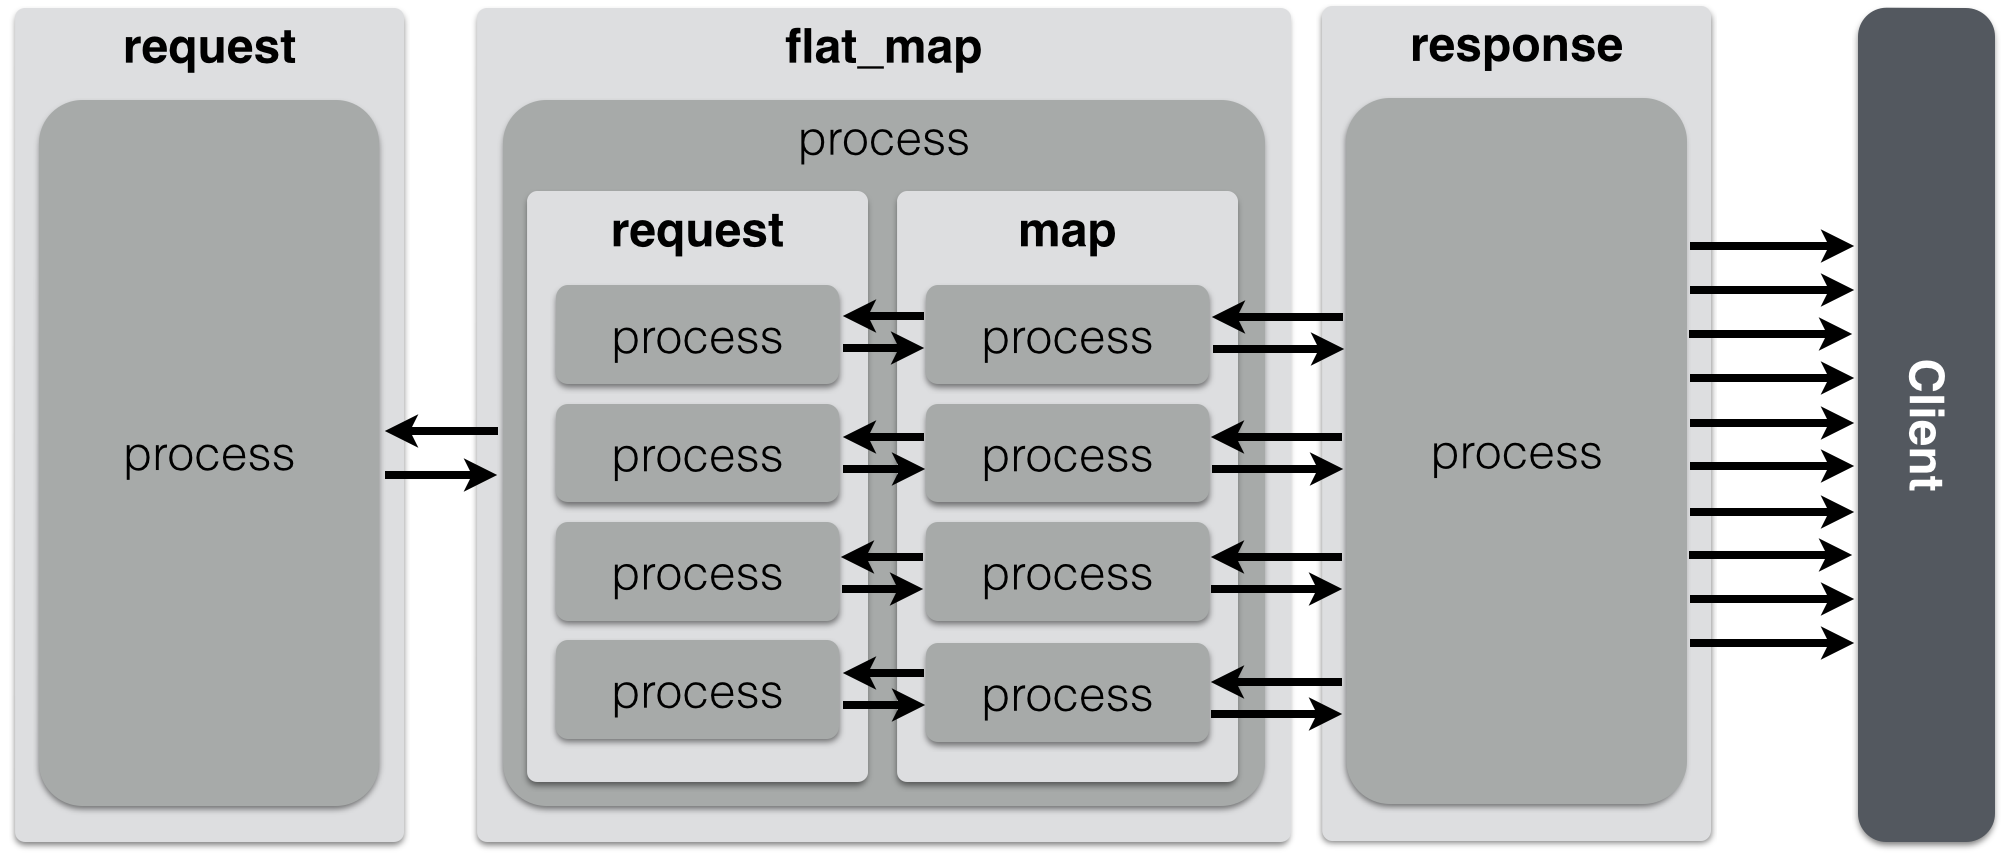
\includegraphics[width=0.9\textwidth]{images/process_overview.png}
    \end{center}
  \caption{Sketched overview of how the processes communicate in the middle pipeline defined in Figure~\ref{fig:complete_end_point}, line 6--35.}
  \label{fig:process}
\end{figure}

When we call the first \lstinline{request} function on line 7, it will spawn a new process which will execute the HTTP request to the defined URL. We then we call \lstinline{flat_map} on line 8 and it will spawn a matching new process which will send a message to the process defined in \lstinline{request} telling it that it is ready to receive data as soon as it is ready (as soon as the HTTP request is done). When the HTTP request is done, the process in \lstinline{request} will send the results to the process defined in \lstinline{flat_map}.

A new pipeline is created inside the \lstinline{flat_map} function's process---spawning a process inside another process means that the internally defined processes has access to the outer process's data via the scope. 

On line 22, we call \lstinline{request} with a list of URLs. The internal \lstinline{request} function will spawn a new process for each URL so that each HTTP request will be executed by a unique process. When we call \lstinline{map} on line 23, it knows how many processes that have been spawned inside \lstinline{request}, and thus, it will spawn the same amount of new processes to receive the data and transform it.

The \lstinline{response} function defined in the outer pipeline will spawn just one new process even though it will communicate with an arbitrary amount of processes. This is because its job is to create one HTTP response by consolidating the responses from all processes.

It is important to understand that the arrows drawn in Figure~\ref{fig:process} are independent of each other and that they are not ordered in any way. We can think of the arrows as open roads where the messages race like cars to the finish line---the processes spawned by the \lstinline{request} function defined inside \lstinline{flat_map} are independent of each other, the first responding HTTP request has the opportunity to be sent first to the client.

\section{Related works}
\subsubsection{Tyk}

Tyk is an open source API gateway written in Go which enables you to control who accesses your API, when they access it and how they access it. It can, like Rackla, transform requests but it uses templates instead of code. This approach can make the end-point development easier with the downside of being less powerful.

\vspace{5mm}

\noindent \url{https://tyk.io/}

\subsubsection{LoopBack-Gateway}

LoopBack-Gateway is an experimental, minimum viable product, API gateway developed by StrongLoop. It is written in JavaScript using Node.js and focuses on rate limiting, reverse proxying and security.

\vspace{5mm}

\noindent \url{https://github.com/strongloop/loopback-gateway}

\chapter{Cases studies}

Three systems were evaluated in order to find potential usage areas for API gateways in real-world products. The goal was to look at the three systems from different view points; if two systems have a common problem, then it will only be mentioned in one of the case studies. The reasoning behind this was to highlight the different usage potential for API gateways.

\section{Streamflow}
Streamflow\cite{streamflow} is a system used within municipalities in order to communicate with its citizens and inside organisations to communicate with their customers. It is primarily used to register and track customer cases and works as a central case management hub.

Streamflow exposes a HATEOAS REST API with JSON-encoded responses. The desktop client for Streamflow was written in Java using Swing---however, a new web-client written using AngularJS, a JavaScript Framework developed by Google, is currently under development. The following case study used the in-development AngularJS client with the current production API over HTTP/1.1.

\subsection{Case lists}
In Streamflow, incoming cases are automatically categorised according to rules defined by the municipality or organisation. Each category has two folders: \enquote{inbox} and \enquote{my cases}. When clicking on the \enquote{inbox} or \enquote{my cases} for a category, all cases in that folder will be fetched from the server and the results will be displayed in a list.

\subsection{Evaluation}
When viewing the case list, several recursive requests will be executed from the client in order to collect all the required information and in order to follow the HATEOAS specification (the first steps in the request chain has been omitted):

\begin{enumerate}
	\item Request a list of all cases in the selected category and folder. This will return a list of case-objects which are 0.9~KB per object.
	\item For each case in the list, request the case information. This will return the same case-object once more with additional meta data. The reason for executing this request is to discover the next hypermedia resource called \enquote{general}. The wanted payload, the \enquote{general} resource, is 94~bytes while the total response is 3.5--4~KB. This results in a overhead of roughly 97.5\% unnecessary data for each request.
	\item Request the \enquote{general} resource for each case. From this response, the client wants two fields: a date and a note. If a priority is present, the client also wants the next resource called priorities. The total response is 1.5--2~KB and the wanted data is 130~B resulting in a unwanted overhead of roughly 92.5\% for each request.
	\item If the cases has a defined priority, that priority has to be requested. This response is 293~B and will contain information about all priority levels, usually four levels. A case can only have one priority which results in a 75\% overhead for each request.
\end{enumerate}

\begin{figure}[H]
  \centering
    \begin{center}
      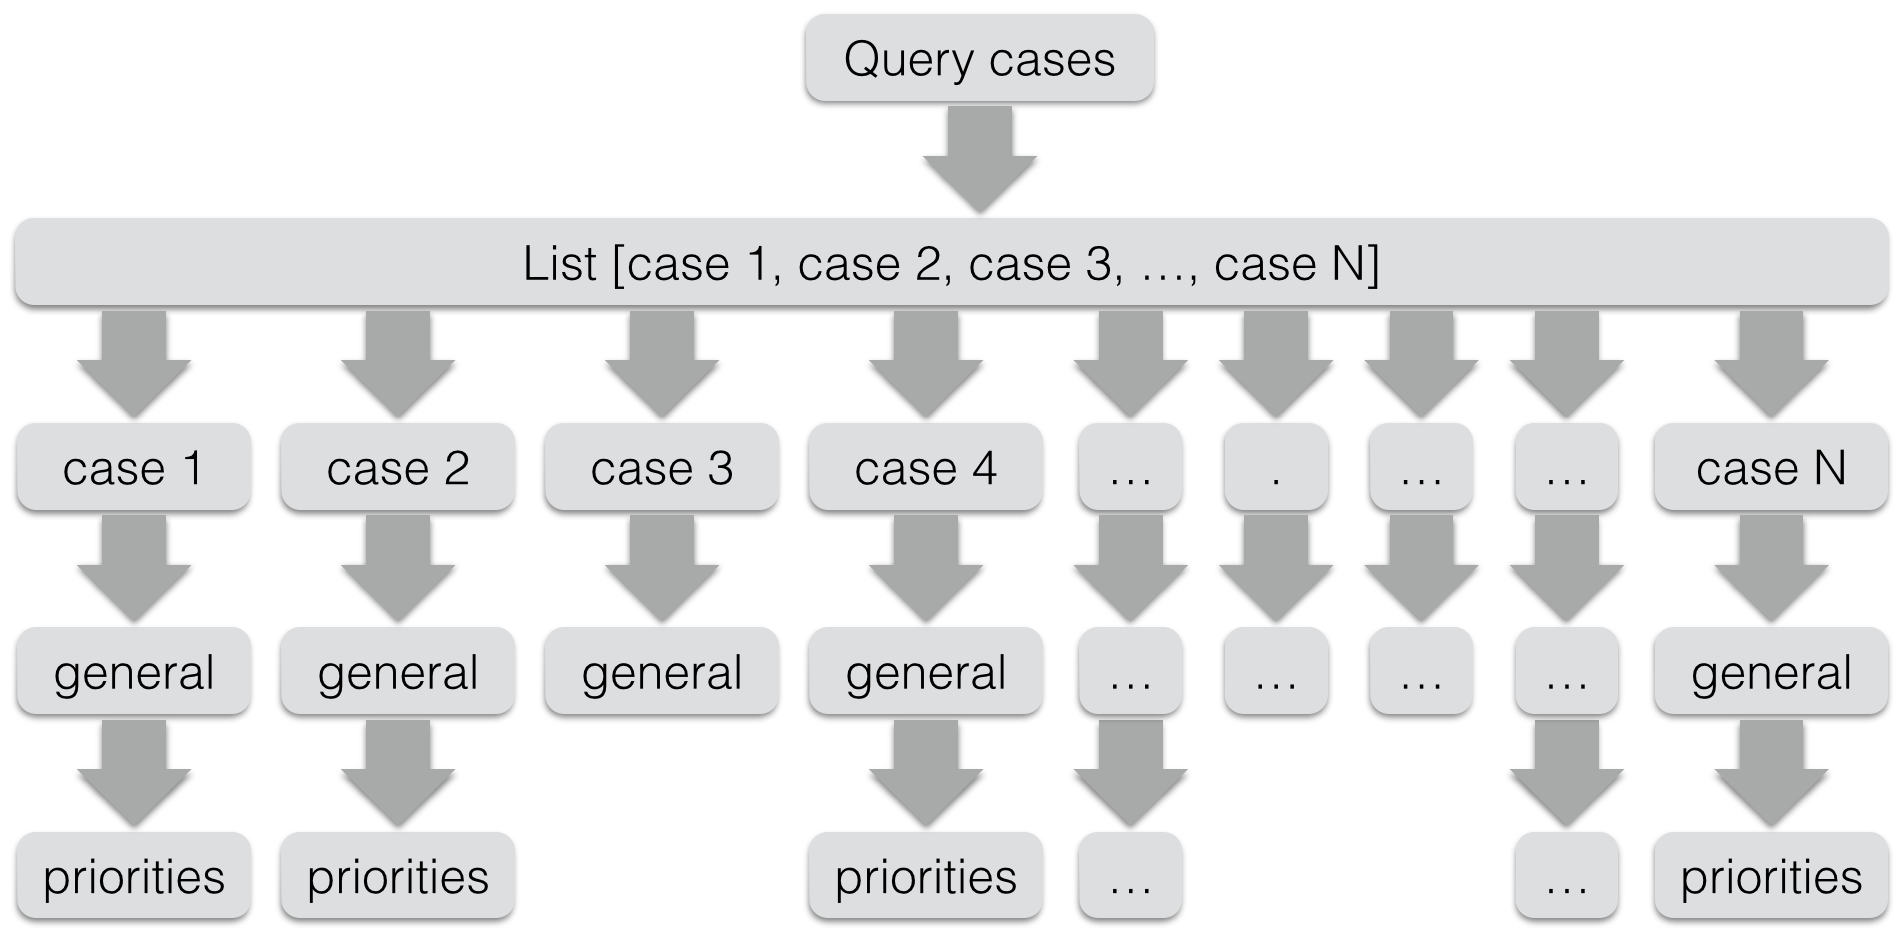
\includegraphics[width=0.9\textwidth]{images/streamflow_cases.png}
    \end{center}
  \caption{How the recursive requests are executed in the Streamflow web client in order to fetch all needed resources and to comply with HATEOAS in the REST architectural specification.}
\end{figure}

By placing an API gateway developed with Rackla between the Streamflow web-client and the Streamflow API, all recursive requests can be concatenated, for the client, to one request with a single response. By doing so, a lot of unnecessary data can also be discarded before it is sent to the client. This unnecessary data is duplicate data such as the duplicate case-information, irrelevant data for the client such as HATEOAS discovery information and unneeded data such as unused priorities.

In the test environment, measurements were made on a list which contained 156 cases. For this list, the client had to execute 373 requests: 1 request for the list, 156 requests for each case to get the location of the \enquote{general} resource, 156 requests for the \enquote{general} resource for each case, and 60 \enquote{priority} requests for the cases which needed that information. All these request where replaced with one single request to the API gateway which took care of the HATEOAS communication. By doing so, the total transmitted data was reduced from 1,100~KB to 159~KB---a 86\% decrease of transmitted data.

The Streamflow API does not compress any of the responses. By adding Gzip compression to the payload inside the API gateway before responding to the client, the data could be reduced even more, from 1,100~KB to 9.9~KB, which amounts to a 99\% decrease of transmitted data.

In addition to this, the client also had to transform certain data types after retrieving them from the server so that it would fit in its internal model. For example, the field \enquote{dueOn} was truncated from \enquote{2015-02-17T23:59:59.000Z} to \enquote{2015-02-17} since the time part was not relevant for the client. By utilising the API gateway, these transformations could be taken care of before replying to the client. This means that no, potentially demanding and error prone, transformations had to be performed on the client---instead the data from the response could be used directly.

\begin{figure}[H]
  \centering
    \begin{center}
      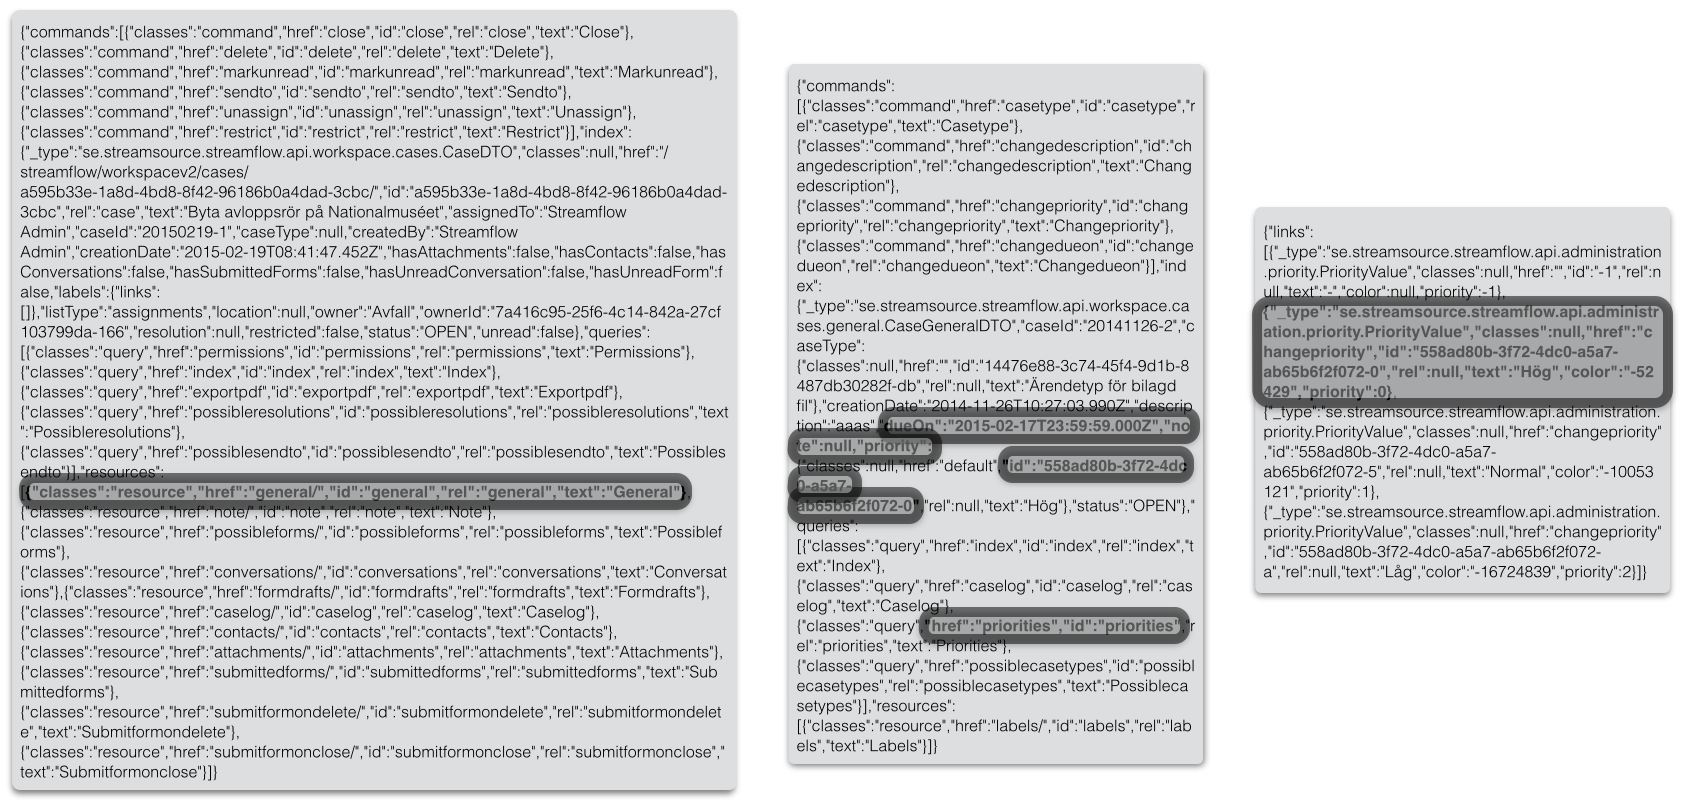
\includegraphics[width=0.9\textwidth]{images/streamflow_response.png}
    \end{center}
  \caption{Illustration of the responses (case, general and priorities) from Streamflow. The actual data needed in the list view is highlighted in order to illustrate how much unnecessary data that was transmitted.}
\end{figure}

In the production environment, a measurement was made in order to determine the number of cases present in the municipality of Jönköping at a given time of the day. On average, the number of cases in the non-empty inboxes was 19 and the maximum number of cases in one inbox was 296. This means that on average, the number of requests performed, every time an inbox is checked from the client, is roughly 40--60. When the largest inbox is viewed, the number of requests will be somewhere between 600--900---every time it is clicked. This is a substantial performance bottleneck for all clients, especially browsers using HTTP/1.1 considering the TCP max-connection limit and the various textual overheads.

It should be noted that the final version of the web-client will most likely be limited to displaying 10--20 cases at a time using pagination. This would reduce the number of requests to 20--60 for any given inbox view. This is however still a substantial amount of HTTP requests to perform every time a user checks an inbox. This approach will neither address the problem that 86\% of the transferred data is unnecessary overhead.

\section{Bank App}
The second system evaluated was a banking app for an undisclosed major bank in Sweden, here after simply called \enquote{Bank App}. Bank App is a mobile app with clients for iOS, Android and Windows Phone. What made the Bank App interesting, from the API gateway point of view, was that it already had a modern and well designed API, which was adapted to the needs of the clients, from the start. Additionally, the clients were written as hybrid apps in which common web technologies could be shared among the different platforms and only a small amount of native components had to be rewritten.

\subsection{Transaction overview}
An essential part of the application is the transaction overview which is where the users can view their balance, orders, fund orders, trades and transactions.

When the transaction overview screen is loaded, the client uses promises (asynchronous computations) to collect and transform the results from the different back-end API end-points. The results are then bound to the scope variable which in turn makes sure that the information is rendered in the view.

\begin{figure}[H]
  \centering
    \begin{center}
      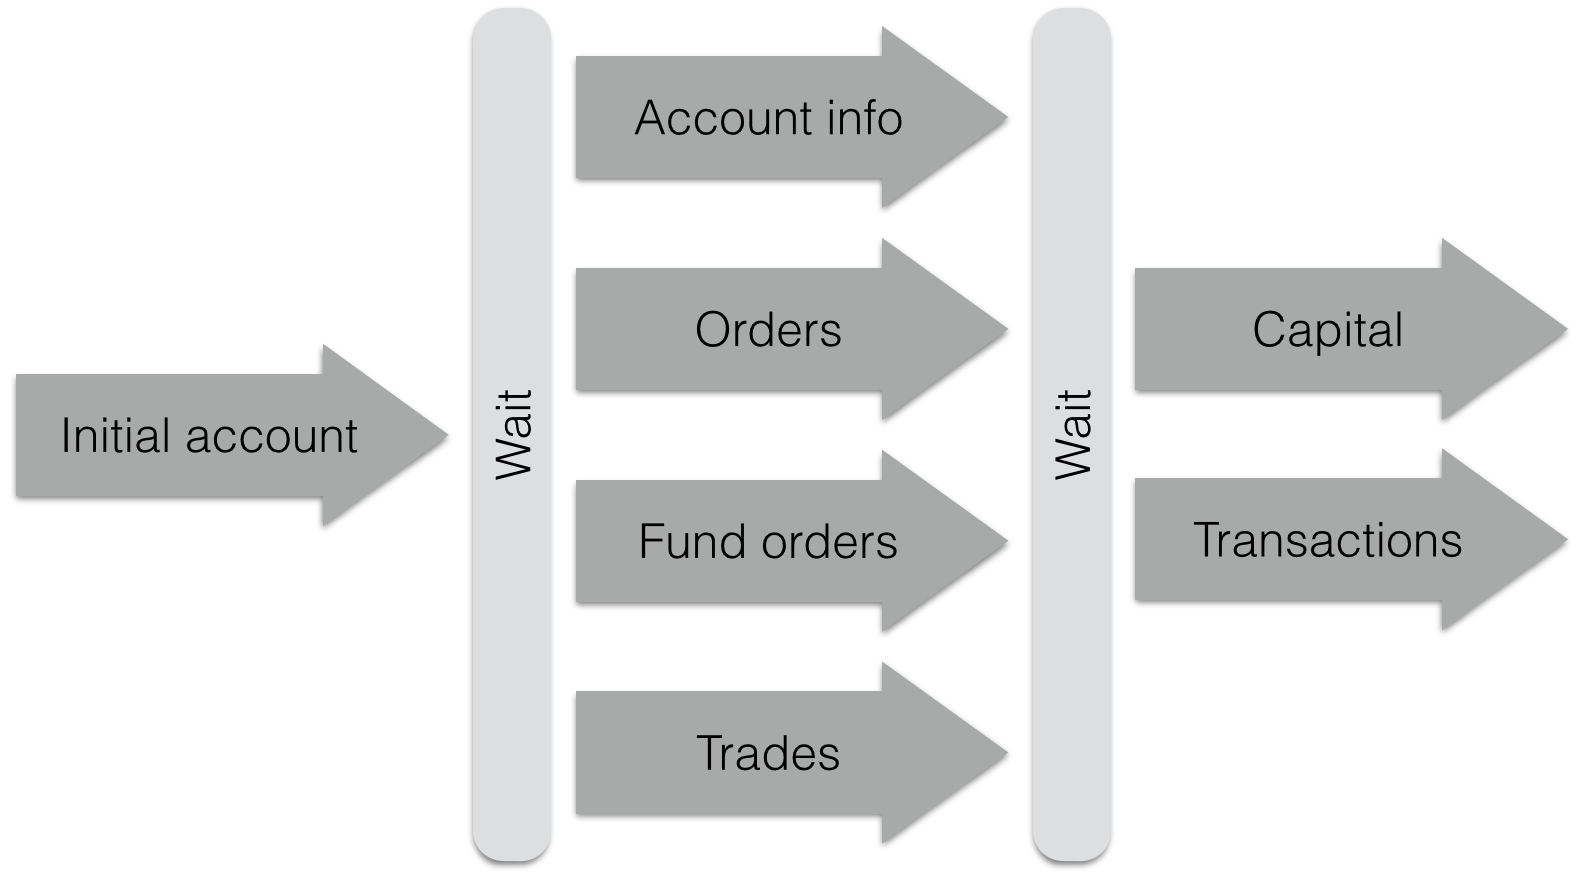
\includegraphics[width=0.9\textwidth]{images/bank_overview.png}
    \end{center}
  \caption{How the asynchronous calls to the API and the transformation works. There are two places where the code waits for previous computations before continuing.}
\end{figure}

To load the required data, the initial account information has to be fetched first. Using that response, the client will then load the account information, orders, fund orders and trades for that account. The client then waits for the four requests to respond, perform some transformations to the data and then merge it with capital and transactions data so that the fetched information fits the clients internal data model.

\subsection{Evaluation}
All in all, the client requests data from seven different API end-points and uses about twice as many functions to fetch and transform these results in the transaction overview. Since the number of parallel requests are less than six in the transaction overview, it will have no problem with the TCP-connection limit.

The data served from the API only had a small amount of information which the client discarded and so the data transfer before and after the introduction of the gateway was almost identical---about 1 KB less after the introduction of the API gateway.

It is possible that the overhead of unnecessary data can differ from customer to customer. One example of this is the fact that the API sends all of the customer's accounts, including inactive accounts, but the client is only interesting in the active accounts. It is however hard to argue that this amount of overhead is so substantial that it will cause performance issues.

What made the Bank App special was that the different mobile platforms shared a common code base for the overview screen. This meant that iOS, Android and Windows Phone could utilise the same JavaScript code for transforming, filtering and sorting the requested data.

If the Bank App instead would have been developed using native code, we would see that the fetching and transforming code had to be rewritten for each platform in a new language. If we draw a parallel to the industry average defect rate, about 1--25 errors per 1000 lines of code\cite[page 521]{code_complete}, this means that every new client platform introduced to the transaction overview would potentially create 0.1--2.5 new bugs---a number which could be reduced if the code only had to be written once in the API gateway instead.

Perhaps more importantly, moving the code to the API gateway means that the combined codebase would not just be less error prone but it would also be more maintainable. If we, to take one example, wanted to sort the accounts in descending order rather than ascending, we could change this code once in the API gateway and avoid updating every client. 

If this code was instead located in the clients, all of them had to be updated individually, probably by different teams, and each of them submitted to the various app stores for a potentially long review process.

Having different code bases for common tasks in the clients would also increase the risk of introducing discrepancies by mistake despite the goal of having identically working clients on all platforms.

In the end, the code in the client to perform these requests and transform the results amounted to roughly 100 lines of code and the corresponding end-point in the Rackla API gateway amounted to roughly the same line count.

It is hard to argue for the inclusion of an API gateway in the current state of this project based on the facts that the Bank App already has a shared cross-platform code base and a well suited API with mostly optimised end-points. One can imagine that the need for an API gateway can increase over time if the API is not moving as fast enough or is as flexible as desired and therefore can not meet the clients needs. It is also a possibility that new clients will be introduced later on, clients move to native code bases instead of hybrid technologies or that they will fork the existing cross-platform code base. However, in the current state of the project, the inclusion of an API gateway will not provide any substantial benefit.

\section{Accountant System}

Accountant System is a code name for a system used by a large Swedish accountant firm to help them keep track of important documents, tasks and internal priorities. The client is a single-page web application written in AngularJS which uses an existing legacy back-end API. The back-end API communicates entirely with XML encoded messages over HTTP---but the client only works with JSON internally. Working with JSON in web applications can be considered very beneficial since JSON and its syntax is a subset of the JavaScript language. JSON support is also included in the ECMAScript standard, which JavaScript implements, since version 5\cite{ecmascript_5}. This enables easy (de)serialisation of JavaScript objects to JSON in all modern browsers.

\subsection{Working with XML in JSON clients}
\label{xml_json}

When it comes to converting XML to JSON, and vice versa, there is no standardised approach which can be applied to make the conversions uniform. Even though the formats do solve some of the same problems in regards to data encapsulation, the semantics and features are inherently different and it is therefore impossible to create a 1:1 mapping between the two formats.

In an article from XML.com\cite{xml_json} which was published by O'Reilly Media, a conversion algorithm was developed to highlight some of the issues regarding this topic. One of the examples started with a very simple XML structure defined in Figure~\ref{fig:xml_structure}.

\begin{figure}[H]
  \centering
    \begin{center}
\begin{lstlisting}[breaklines=true,frame=single]
<e>
  <a>some</a>
  <b>textual</b>
  <a>content</a>
</e>
\end{lstlisting}
    \end{center}
  \caption{Simple XML data structure.}
  \label{fig:xml_structure}
\end{figure}

An algorithm was developed to convert the XML-structure to JSON notation. When this algorithm was tested, the first naive approach to convert the structure from Figure~\ref{fig:xml_structure} to JSON would result in the following invalid JSON structure as seen in Figure~\ref{fig:xml_wrong}.

\begin{figure}[H]
  \centering
    \begin{center}
\begin{lstlisting}[breaklines=true,frame=single]
"e": {
  "a": "some",
  "b": "textual",
  "a": "content"
}
\end{lstlisting}
    \end{center}
  \caption{The first attempt to transform XML to JSON. The result is an invalid JSON data structure because of the duplicate key \enquote{a}.}
  \label{fig:xml_wrong}
\end{figure}

The problem with the JSON structure in Figure~\ref{fig:xml_wrong} is that we can not have \enquote{a} as the key in two places in an associative array---\enquote{a} has to be unique. If we try to solve this by converting the values for the key \enquote{a} to a list instead, then we get a syntactical valid JSON structure as seen in Figure~\ref{fig:json_wrong}.

\begin{figure}[H]
  \centering
    \begin{center}
\begin{lstlisting}[breaklines=true,frame=single]
"e": {
  "a": [ "some", "content" ],
  "b": "textual"
}
\end{lstlisting}
    \end{center}
  \caption{The second approach for transforming XML to JSON. The result is a valid JSON structure but the ordering problem has now been introduced.}
  \label{fig:json_wrong}
\end{figure}

However, another problem has been introduced with this approach which is that the element order is no longer perserved. If we would iterate over the values in the XML from Figure~\ref{fig:xml_structure}, we would end up with \enquote{some, textual, content} but when we iterate over our JSON-structure from Figure~\ref{fig:json_wrong} we would end up with \enquote{some, content, textual} which is not the desired result.

\vspace{5mm}
\noindent Based on this, the following conclusion was made by XML.com:

\begin{quote}

\enquote{A structured XML element can be converted to a reversible JSON structure, if all subelement names occur exactly once, or subelements with identical names are in sequence. A structured XML element can be converted to an irreversible but semantically equivalent JSON structure, if multiple homonymous subelements occur nonsequentially, and element order doesn't matter.} \cite{xml_json}

\end{quote}

Note that the algorithm from XML.com is just one approach to solve some of the problem around XML-JSON conversion---there are many additional issues which makes this conversion very complex. As with many things where there is no 1:1 mapping, different library developers and corporations are developing their own standards to handle the conversion.

To humorously illustrate this problem, a tool was created\cite{jsonx_jsonml} which converted JSON to XML with IBM's JSONx\cite{jsonx} standard and then back to JSON from XML with JsonML's\cite{jsonml} standard. These tools follow their own defined conversion standards with different syntactical data. When these conversions are performed recursively with each output added to the others input, you would expect that the formats would stay the same, switching back and forth between JSON and XML---instead the data structure will grow indefinitely until the browser crashes since each format adds their own custom syntactical data to it.

In the end---the point is that converting XML to JSON, and vice versa, is troublesome and since there is no 1:1 mapping, it is handled differently in the variety of libraries used today.

\subsection{Translating XML APIs}
In Accountant System, the XML-JSON conversion was handled in two different ways---one way for requests and one for responses.

\subsubsection{Response}

When working with XML responses from the API, the client utilised a third-party library which converted the XML responses to JSON which then could be used as JavaScript objects in the views, often after some transformations. As in the previous examples, this adds additional complexity to the client which now has to transform the responses before it can handle them properly.

\subsubsection{Request}
More interesting is how the requests are made to the API. When we look at a typical REST end-point which is accessed over HTTP, we first have a HTTP verb such as GET, POST, PUT or DELETE which indicates how the underlying resource should be manipulated. In addition to this, we have an end-point which we communicate with via a URL. Lastly, we add a payload which either contains the data we want to submit or additional parameters which can make the request more specific than what can be expressed by the URL itself.

In the case of Accountant System, we can look at the simplest scenario which is saving a note. To do this, the client has to send the XML data seen in Figure~\ref{fig:xml_account_example} to the back-end.

\begin{figure}[H]
  \centering
    \begin{center}
\begin{lstlisting}[breaklines=true,frame=single]
<SaveNotesRequest>
  <Notes>
    <JPTEXT>This is the actual note.</JPTEXT>
  </Notes>
</SaveNotesRequest>
\end{lstlisting}
    \end{center}
  \caption{XML data used for creating a new note.}
  \label{fig:xml_account_example}
\end{figure}


This XML data has to be sent with a POST HTTP request to a specific URL with ends with \enquote{/note/create}. We can reason about what the purpose of the XML is. From the URL we can deduce where the information should be sent and what information we are sending---a note. We can from the HTTP verb POST see that we want to create a new note and in this case, the URL also contains this information since it ends with \enquote{/create}. The only thing missing to complete this action is the actual payload which is the note content, in this case \enquote{This is the actual note.}.

When working with this API, the XML is entirely redundant from the clients point of view and it does not add any value, but for historical reasons the back-end API can not change. This puts additional strain and a new layer of complexity in every new client which interacts with the API. Not only do the client have to know about the normal interaction methods such as the URL and HTTP verbs but it also needs to maintain a collection of XML templates and use a different XML template for each type of request it wants to execute. It is also worth pointing out that the the actual note amounted to roughly 1/3 of the total payload data and about 2/3 was structural XML data in the example from Figure~\ref{fig:xml_account_example}.

\begin{figure}[H]
  \centering
    \begin{center}
      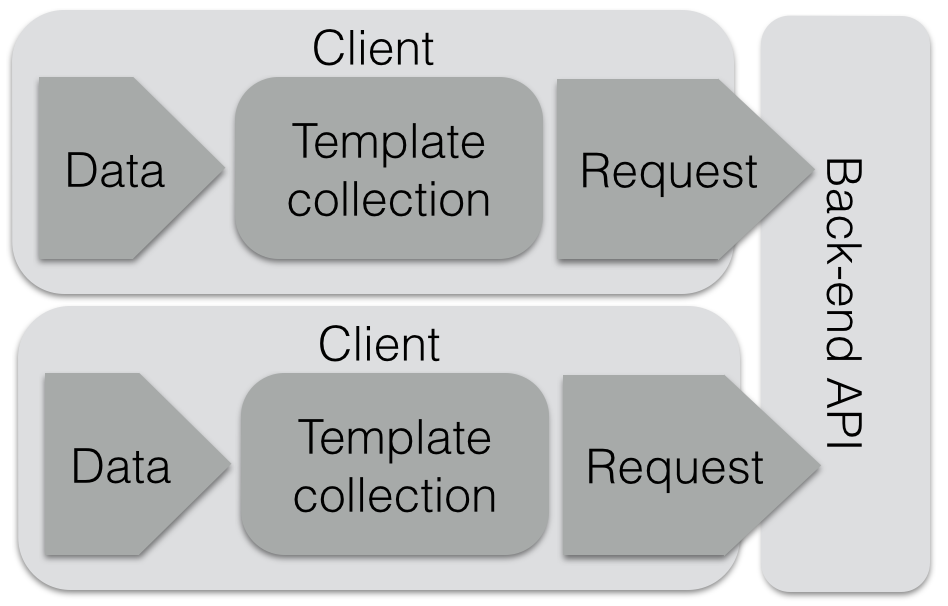
\includegraphics[width=0.7\textwidth]{images/client_templates.png}
    \end{center}
  \caption{Each client has to maintain its own collection of XML templates in order to make requests to the API.}
\end{figure}

To avoid having to maintain a collection of XML templates in each client, we can introduce an API gateway to do that instead. By introducing an API gateway, we can expose corresponding new end-points which can be used without any XML in the client. The API gateway will maintain the only collection of XML templates which it uses for translating the client's API-requests to back-end API requests. This makes the development of clients a lot easier from the API-call point of view but also has the benefit that there is only one, easily maintainable, collection of XML templates.

\begin{figure}[H]
  \centering
    \begin{center}
      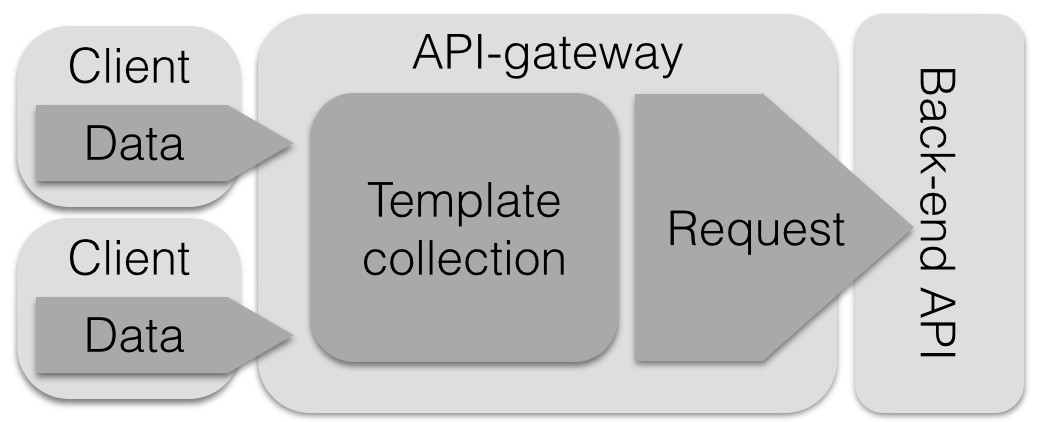
\includegraphics[width=0.7\textwidth]{images/gateway_templates.png}
    \end{center}
  \caption{The API gateway maintains a collection of XML templates so the client can communicate to the back-end without them.}
\end{figure}

\subsection{Evaluation}

In the case of Accountant Software, we can see a decrease in used bandwidth when dropping the XML format in the client since XML is a verbose, an in this case unnecessary, format. It is worth pointing out that the XML templates were not only transmitted upon each request but the entire collection of XML templates also had to be downloaded to the browser every time the single-page application was initially loaded. 

A study in 2011 compared the XML-based protocol SOAP\footnote{Simple Object Access protocol, see appendix.} with FIX (Financial Information Exchange) and CDR (Common Data Representation) in financial messaging systems and concluded that SOAP had 2--4 times larger messages on average\cite{soap_fix}. It is however hard to draw a fair parallel with that study to this case study.

The biggest gain in utilising an API gateway in this scenario is likely to be found in developer productivity and code stability. The JSON versus XML is an ongoing debate which has been active for several years. Jeff Barr who is the Chief Evangelist for Amazon Web Services stated back in 2003 that 85\% of their API users utilised REST while only 15\% wanted the XML-based SOAP interface\cite{soap_amazon}. The comparison here is not entirely fair either since SOAP is a protocol, not just using XML, while REST is an architectural style which can utilise XML---and that is the case for Accountant Software.

What we can do is to look at the limitations in XML for Accountant Software in particular. The first thing to note is that all modern browsers has built in support for a standardised way of parsing JSON and that there is a natural 1:1 relationship between JavaScript objects encapsulating data and the JSON format. For Accountant Software to work with XML, a third-party library was introduced and all API-responses has to be validated to make sure that the JSON-to-XML parsing works in a decent manner as there are pitfalls to watch out for. For clients written in JavaScript, it would be a more natural approach to use an JSON-based API.

An API gateway can, like the client already does, automatically translate the XML-based responses from the API to JSON. The benefit of placing the translation step in the API gateway is that all clients will have translation done in exactly the same way instead of relying on different local translation libraries.

\begin{figure}[H]
  \centering
    \begin{center}
      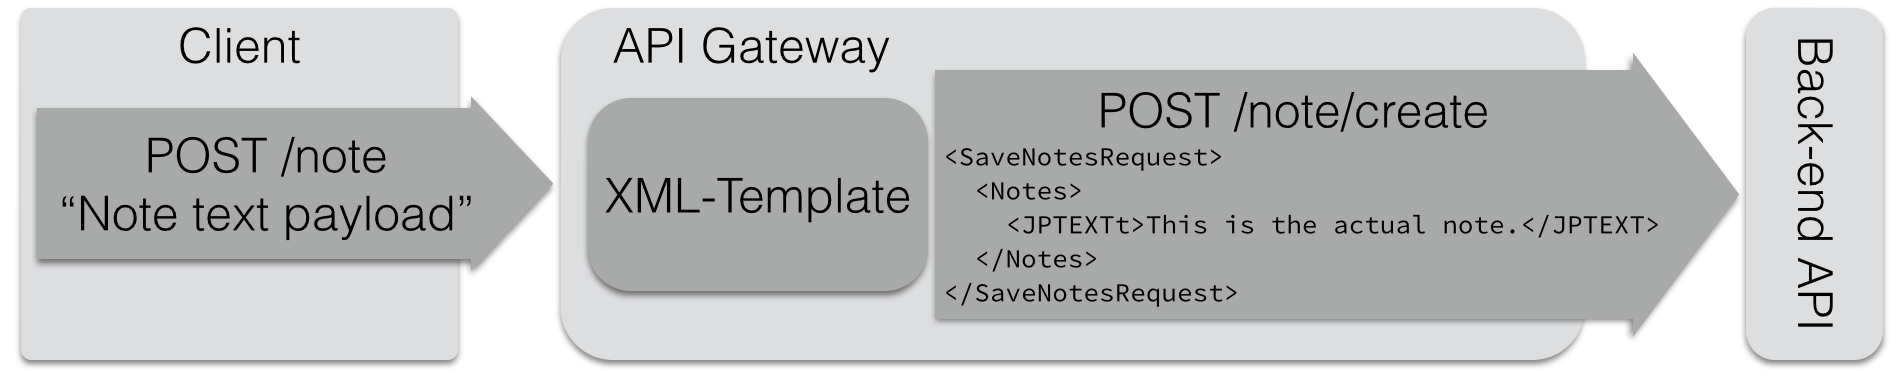
\includegraphics[width=0.9\textwidth]{images/api_gateway_xml.png}
    \end{center}
  \caption{The API gateway exposes a simpler REST interface to the client and converts this to the more complex XML-based interface to the back-end.}
\end{figure}

When looking at the requests the client sends to the back-end API, we earlier concluded that the XML in many cases was unnecessary since all information describing data was already present in the URL in combination with the HTTP verb. By moving all XML-templates to the API gateway, all clients can utilise a much simpler API. An additional benefit to this approach is that all XML-templates are gathered in one place in contrast to the current approach where every client has to keep track of their own collection of templates.

\chapter{Conclusions}
As seen in the case studies, the API gateway concept is not a silver bullet and the need for an API gateway varies on a number of factors such as which technology is used in the client and the back-end servers, and how well the API can be adapted to the clients' needs. We have also seen that API gateways can be used for many different purposes---from network performance improvements to reducing code complexity and increasing developer productivity.

Requests are still \enquote{expensive} in HTTP/1.1 because of the substantial amount of overhead from headers and cookies, and the TCP connection limit. Browsers are limiting the TCP connection pool to six connections which degrades the performance, especially when the network connection is suffering from a high latency. HTTP/2 will solve many of these issues but a complete switch to HTTP/2 will take at least a decade\cite[page 21]{hpbn2} ---the change will not only be demanding for the browser and server developers but all intermediate devices such as proxies has to be upgraded as well. The HTTPbis working group has also announced that HTTP/2 will only work with URLs protected with SSL (HTTPS)\cite{http2_ssl}. This will likely slow down the HTTP/2 adoption rate which further highlights the need for an optimising API gateway for many years to come. Simple techniques such as request concatenation and data transformations can dramatically increase the performance when looking at the communications between the clients and back-end servers.

We have in the case studies seen that API gateways can be very useful when working with legacy back-end APIs that does not conform to the clients' needs. There are many scenarios where the back-ends themselves can not be changed such as when old clients has to be supported or the back-end itself is not actively developed. In such scenarios, API gateways can move the burden away from the clients by placing it close to the back-end, where the network costs are negligible, and letting it do all the work. 

The API gateway is not only useful for optimising performance but can also increase developer productivity. By transforming the responses to the format which the clients can handle the best, the API gateway can make the client development process easier and less error prone while also boosting developer productivity.

API gateways can also be useful when designing new systems which has to support a variety of clients. This has been noticed in the architectural design implemented at Netflix\cite{netflix} which must support many different clients with different needs. In the case of Netflix, the client teams are responsible for developing their own end-points which serves their client a custom tailor-made response. This approach puts the same amount of work on the client and back-end developer teams but lessens the traffic costs, reduces the clients complexity and can increases overall performance.

\section{Future work}

The API gateway concept is very broad and there are many unexplored areas to which the concept can be applied. There are many topics in this thesis which are only briefly touched upon, such security and caching, which could fill an entire thesis of their own in order to be fully explored.

The framework Rackla developed in this thesis used Elixir but there is no doubt that the same functionality could be translated to many other programming languages as well. By migrating the framework to other languages, new challenges and solutions would doubtless appear and shine new light on the topic. 

\cleardoublepage
\phantomsection
\addcontentsline{toc}{chapter}{Bibliography}
\bibliographystyle{unsrt}
\bibliography{anton_msc}

\begin{appendices}
\chapter{Definitions}
\section{JSON}
JSON, JavaScript Object Notation, is a data-interchange text format based on a subset of the JavaScript Programming Language. It is an open standard format which uses human-readable text. JSON is often used as an alternative to XML.

\section{XML}
XML, Extensible Markup Language, is a markup language used for encoding documents. It can be used as an alternative to JSON for data communication but it is also used in other areas and document formats.

\section{REST}
REST, Representational State Transfer, consists of guidelines and best practices for creating scalable web services. The style was developed by the W3C Technical Architecture Group (TAG) in parallel with HTTP/1.1. RESTful systems often communicate over HTTP using so called HTTP verbs such as GET, POST, PUT and DELETE to send and retrieve data between clients and servers.

\section{HATEOAS}
HATEOAS, Hypermedia as the Engine of Application State, is a constraint in the REST architecture. The clients enter a REST application through a fixed URL and all future actions are discovered dynamically within resource representations sent from the server.

\section{DMZ}
DMZ, DeMilitarised  Zone, is an isolated subnet located outside the protected LAN where workstations and internal back-end systems are located. It is common that machines, which have to be directly exposed from the internet, are placed inside the DMZ.

\section{SOAP}
SOAP, Simple Object Access protocol, is an XML-based protocol used for data exchange. SOAP is primarily transported using HTTP but can also be used with other protocol such as the e-mail protocol SMTP.

\section{Proxy}
A proxy server acts as the intermediary between clients and servers by relaying the data between them.

\section{LAN}
LAN, Local Area Network, is a network limited to a smaller area such as a building or an office.

\section{WAN}
WAN, Wide Area Network, is a network consisting of a large region such as a country or many countries. The internet is considered to be a WAN.

\section{VPN}
A VPN, Virtual Private Network, is used to securely extend a private network, such as the network inside a corporation, to an outside public network such as the internet.

\end{appendices}

%\makebibliography{anton_msc}

\end{document}